%!TEX root = ../thesis.tex
%*******************************************************************************
%*********************************** Experiment *****************************
%*******************************************************************************

\chapter{Experiment} 

\ifpdf
    \graphicspath{{chapter-experiment/Figs/Raster/}{chapter-experiment/Figs/PDF/}{chapter-experiment/Figs/}}
\else
    \graphicspath{{chapter-experiment/Figs/Vector/}{chapter-experiment/Figs/}}
\fi


One of Europe's first joint ventures in science~\cite{About:1997225}, CERN (Conseil Européen pour la Recherche Nucléaire) is the largest physics research facility in the world, bringing together more than \num[group-separator={,}]{12200} people from of 110 nationalities to work together and push the frontiers of science and technology. Located at the Franco-Swiss border near Geneva, CERN was founded in 1954 and nowadays counts 23 member states~\cite{About:1997225}. CERN's main research area is particle physics, hence why the organization operates a full complex of particle accelerators and detectors.

This chapter introduces the \gls{lhc}, CERN's main particle accelerator, as well as the ATLAS experiment, in which the \gls{susy} search presented in this work is embedded in.

\section{The Large Hadron Collider}\label{sec:lhc}

The LHC~\cite{Evans:1129806} is the largest particle accelerator situated at CERN. It is installed in a tunnel with $\SI{26.7}{\km}$ circumference, that was originally constructed from 1984 to 1989 for the \gls{lep} accelerator. The tunnel is situated on the Franco-Swiss border and wedged between the Jura mountains and lake Léman. It lies between $\SI{45}{\meter}$ (in the limestone of the Juar) and $\SI{170}{\meter}$ (in molasse rock) below the surface, resulting in a tilt of $1.4\%$ towards the lake.  While proton-proton ($pp$) collisions are the main operating mode of the \gls{lhc}, its design also allows it to accelerate and collide heavy ions like lead and xenon. Since data from $pp$ collisions is used in this work, the following sections will mainly focus on this operating mode. As a particle-particle collider, the \gls{lhc} obviously consists of two rings with counter-rotating beams, as opposed to particle-antiparticle colliders that only need a single ring. With an inner diameter of only $\SI{3.7}{\meter}$, the tunnel however simply too narrow to fit two separate proton rings. Instead the \gls{lhc} is built in a twin bore design\footnote{Originally proposed by John Blewett at BNL for cost-saving measures of the Colliding Beam Accelerator~\cite{Evans:1129806}.}, housing two sets of coils and beam channels in a single magnetic and mechanical structure and cryostat~\cite{Evans:1129806}. While saving costs, this design has the disadvantage of both beams being magnetically coupled, thereby reducing flexibility of the machine. 

Before being injected into the LHC, protons are pre-accelerated by an injection chain built from multiple existing machines in CERN's accelerator complex, pictured in \cref{fig:accelerator_complex}. The injection chain consists of predecessor accelerators that have been upgraded in order to be able to handle the high luminosity and high energy requirements of the \gls{lhc}. The protons for the \gls{lhc} stem from a duoplasmatron source~\cite{Scrivens:1382102}, stripping electrons from hydrogen atoms through electric discharges between a hot anode and cathode. The $\SI{90}{\keV}$ protons are then accelerated by a \gls{rf} quadrupole to $\SI{750}{\keV}$ before being injected into Linac2\footnote{Originally built to replace Linac 1 in order to produce higher energetic proton beams, Linac 2 has been replaced by Linac 4 in 2020.}, a linear accelerator producing a beam of $\SI{50}{\MeV}$ protons through the use of \gls{rf} cavities. The protons then enter a set of circular accelerators, the Proton Synchrotron Booster, the Proton Synchrotron and the Super Proton Synchrotron, creating a stepwise acceleration up to an energy of $\SI{450}{\GeV}$, which is the injection energy of the \gls{lhc}. The \gls{lhc} finally accelerates the protons up to nominal beam energy before colliding them. 

\begin{figure}
	\centering    
	\includegraphics[width=0.9\textwidth]{CCC-v2019-final-white}
	\caption[CERN accelerator complex]{CERN accelerator complex as of 2018~\cite{Mobs:2684277}.}
	\label{fig:accelerator_complex}
\end{figure}

The \gls{lhc} is composed of eight straight sections and eight arcs. The eight straight sections each serve as interaction points (\textit{Point}), either for particle detectors, or for machine hardware of the collider itself. The Points are labelled clockwise, with IP 1 being closest to the CERN Meyrin site. Four of the eight Points house the main particle physics experiments at the LHC, called ATLAS, CMS, ALICE and LHCb, covering a wide range of fundamental research. The two general purpose particle detectors ATLAS~\cite{Aad:2008zzm} and CMS~\cite{Chatrchyan:2008aa} are installed at Point~1 and Point~5, respectively. Both ATLAS and CMS are designed to perform high precision SM measurements including Higgs measurements as well as searches for BSM physics. Being very similar in terms of targeted phase space, ATLAS and CMS can be used to cross-check results of each other. ALICE~\cite{Aamodt:2008zz} is situated at Point~2 and specializes on heavy ion physics, studying the physics of quark-gluon plasma at high energy densities. Built in Point~8, LHCb~\cite{Alves:2008zz} targets $B$-physics and performs measurements of CP-violation. Apart from the four main experiments, three smaller experiments exist at the \gls{lhc}: TOTEM, MoEDAL and LHCf. While TOTEM~\cite{Anelli:2008zza} and LHCf~\cite{Adriani:2006jd} study forwards physics close to CMS and ATLAS, respectively, MoEDAL~\cite{Pinfold:2009oia} searches for magnetic monopoles.

The remaining four Points house accelerator equipment needed for operation of the LHC. Most of the collimation system is placed at Point~3 and Point~7, performing beam cleaning and machine protection through a series of beam intercepting devices, ensuring that no stray particles from experimental debris or beam halo can reach and damage other machine components. The acceleration of the beam itself is performed at Point~4 with two \gls{rf} systems, one for each \gls{lhc} beam. The \gls{rf} cavities operate at $\SI{400}{\MHz}$ and provide $\SI{8}{MV}$ during injection and $\SI{16}{MV}$ during coast~\cite{Evans:1129806}. Due to the \gls{rf} acceleration, the accelerated protons are grouped in packages called \textit{bunches}, each containing roughly $10^{11}$ protons, with a bunch spacing of $\SI{25}{ns}$~\cite{Evans:1129806}. Each beam contains a total of 2808~\cite{Evans:1129806} bunches as design value. The remaining Point~6 houses the beam dumping system, allowing to horizontally deflect and fan out both beams into dump absorbers using fast-paced \textit{kicker} magnets. The two nitrogen-cooled dump absorbers each consist of a graphite core contained in a steel cylinder, surrounded by $\SI{750}{\tonne}$ of concrete and iron shielding~\cite{Bruning:782076}. Insertion of the beams from the Super Proton Synchrotron into the \gls{lhc} happens at Points~2 and 8, close to the ALICE and LHCb experiments.

The eight arcs of the \gls{lhc} are filled with dipole magnets built from superconducting NbTi Rutherford cables. The electromagnets are responsible for keeping the accelerated particles on their circular trajectory and are the limiting factor of the maximal centre-of-mass energy $\sqrt{s}$ of the \gls{lhc}. In order to achieve the design energy of $\sqrt{s} = \SI{14}{\TeV}$~\cite{Bruning:782076}, the magnets have to create a field strength of $\SI{8.3}{T}$~\cite{Evans:1129806}. In order to sustain the electric currents needed for such high field strengths, the magnets need to be cooled down to $\SI{1.9}{K}$~\cite{Evans:1129806} using superfluid helium and operated in superconducting state. In addition to the dipole magnets, the arcs contain quadrupole magnets used to shape and focus the beams, as well as multipole magnets correcting and optimizing the beam trajectory. Quadrupole magnets are also used to reduce the beam size before and after the interaction points.

\subsection{Pile-up}\label{sec:pileup}

\begin{figure}
	\centering
	\begin{subfigure}[b]{0.45\linewidth}
		\centering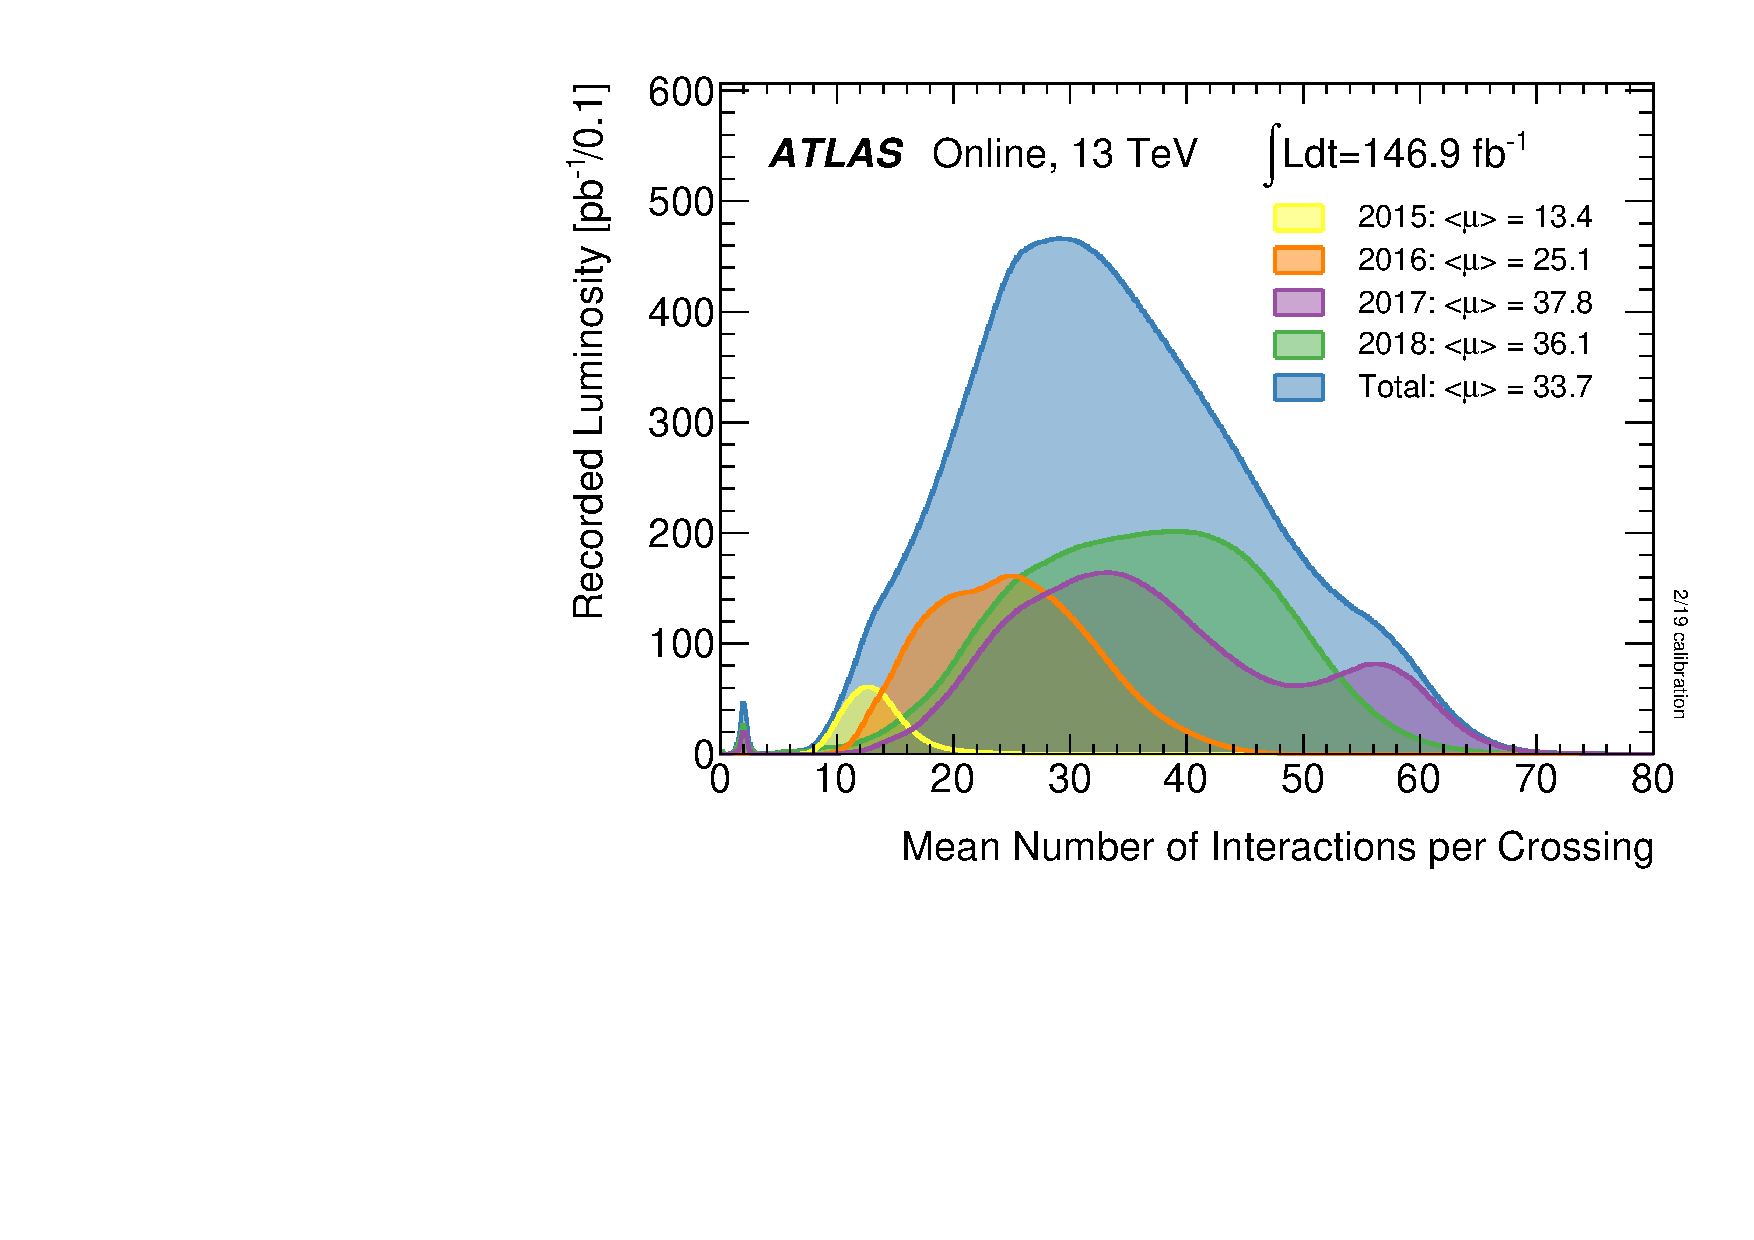
\includegraphics[width=\textwidth]{mu_2015_2018}
		\caption{Luminosity-weighted mean number of interactions per bunch crossing during Run~2 data-taking.\label{fig:mu_2015_2018}}
	\end{subfigure}\hfill
	\begin{subfigure}[b]{0.45\linewidth}
		\centering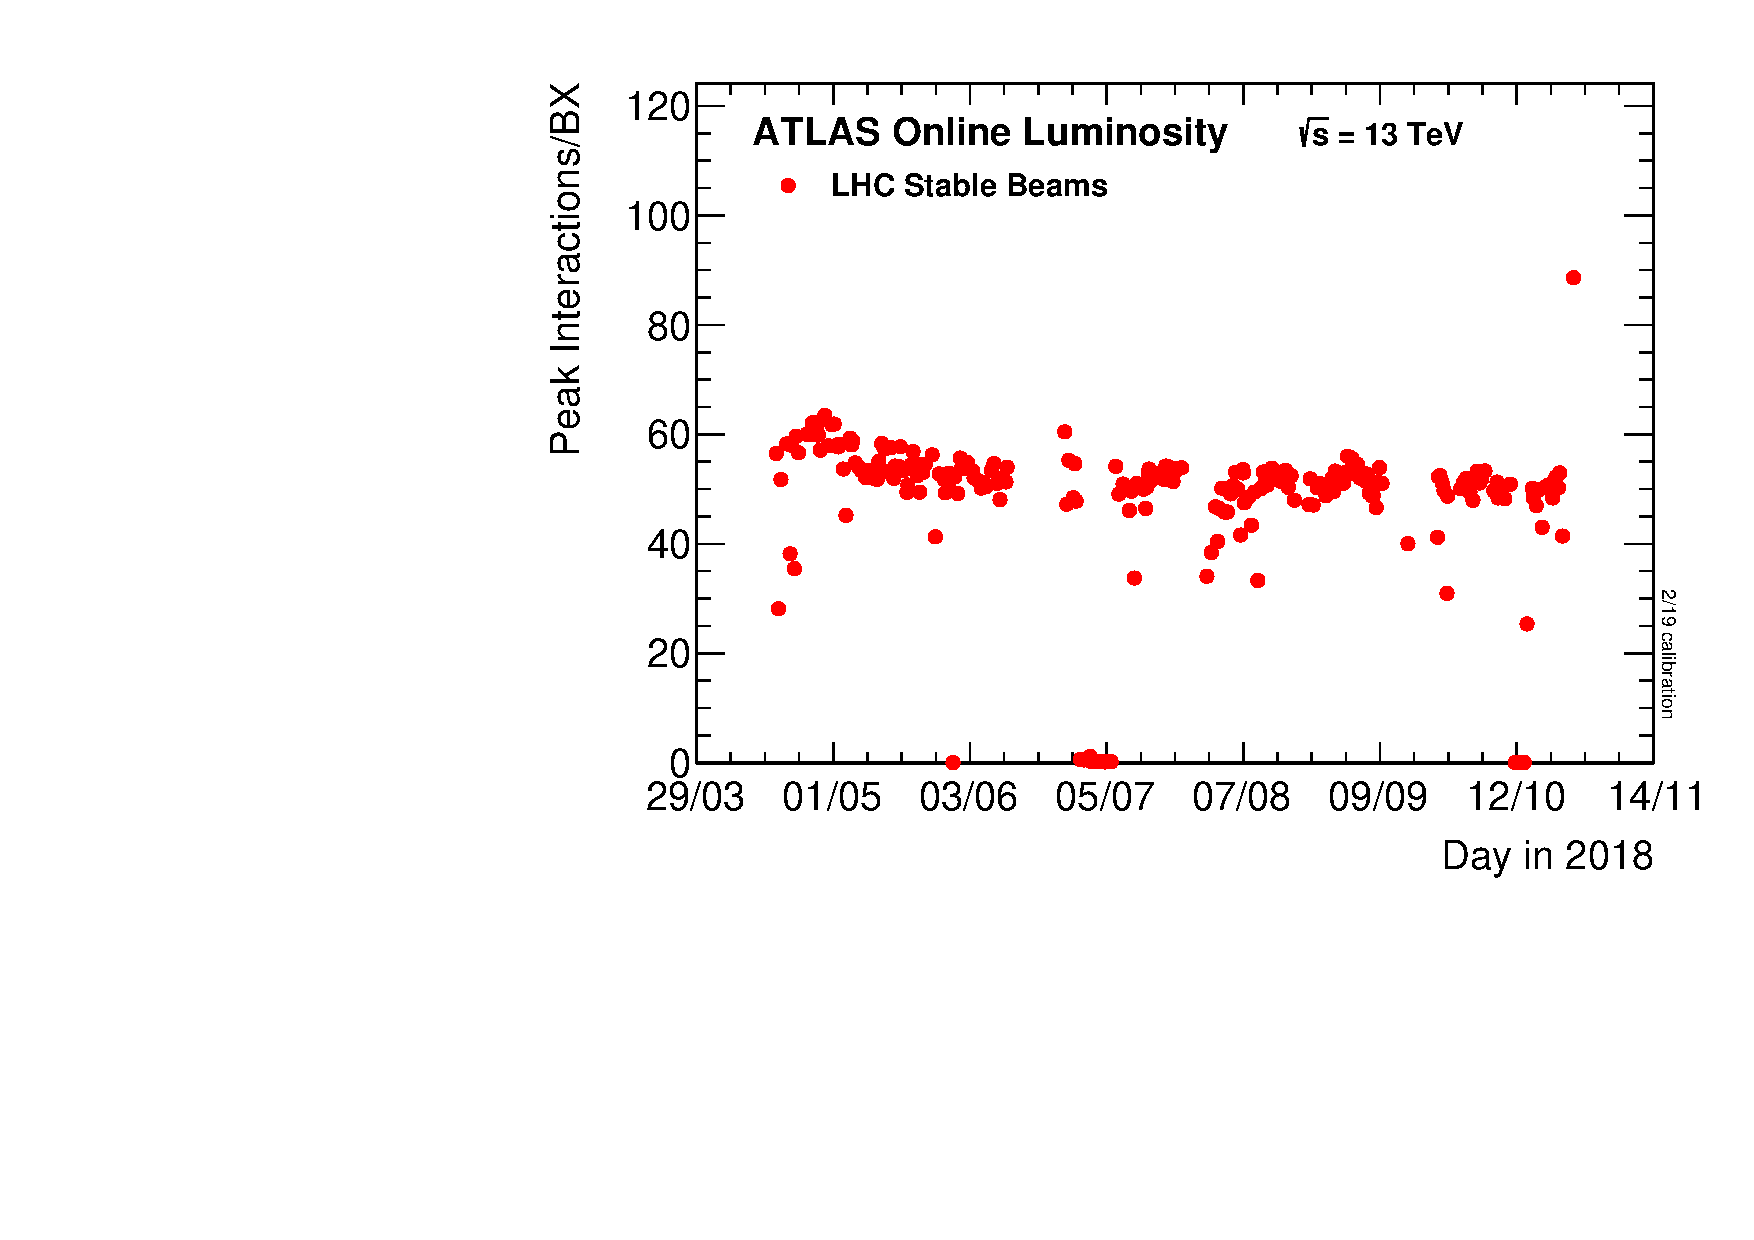
\includegraphics[width=\textwidth]{peakMuByFill}
		\caption{Peak mean number of interactions per bunch crossing for each fill during 2018.\label{fig:peakMuByFill}}
	\end{subfigure}%
	\caption{Number of interactions per bunch crossing recorded by the ATLAS detector~\cite{ATLAS:Run2}}\label{fig:mu_run2}
\end{figure}

Due to the high number of protons in each bunch, several $pp$ collisions occur at each bunch crossing. This leads to a phenomenon called \textit{pile-up}, where the recorded events not only contain information from the hard-scattering process of interest, but also remnants from additional, often low-energy, $pp$ collisions. During the Run~2 data-taking period, the mean number of inelastic $pp$ collisions per bunch crossing, $\mu$, has varied from roughly 10 to 70, with the majority of bunch crossings having a value of $\mu$ around 30. \Cref{fig:mu_2015_2018} shows the mean number of interactions per bunch crossing during the Run~2 data-taking period, weighted by luminosity. The peak number of interactions per bunch crossing $\mu_\mathrm{peak}$ per fill has been consistently around 50 during the 2018 data-taking (cf.~\cref{fig:peakMuByFill}).

Experimentally, pile-up can be divided into five major components~\cite{Marshall:2014mza}:
\begin{itemize}
	\item \textit{In-time} pile-up: multiple interactions during a single bunch crossing, of which not all will be interesting, as often with relatively low energy. If they can be resolved, the main hard-scattering event can still be isolated and studied.
	\item \textit{Out-of-time} pile-up: additional collisions occurring in bunch crossings before or after the main event of interest. This happens either due to read-out electronic integrating over longer time frames than the $\SI{25}{ns}$ bunch spacing, or detector components being sensitive to several bunch crossings.
	\item \textit{Cavern background}: gas of thermal neutrons and photons that typically fill the experimental caverns during a run of the LHC and tend to cause random hits in detector components.
	\item \textit{Beam halo events}: protons scraping an up-stream collimator, typically resulting in muons travelling parallel to the beam pip
	\item \textit{Beam gas events}: collision events that originate from interactions between proton bunches and residual gas inside the beam pipe.
\end{itemize}
While the effects of cavern background can be mitigated through special pieces of shielding, beam halo and beam gas events leave signatures that can be recognized and removed. Signals from in-time and out-of-time pile-up create irreducible overlap with the events of interest, significantly impacting analyses, and thus need to be simulated~\cite{Marshall:2014mza}.

\subsection{Luminosity and data-taking} \label{sec:lumi_datataking}

\begin{figure}
	\centering
	\begin{subfigure}[b]{0.45\linewidth}
		\centering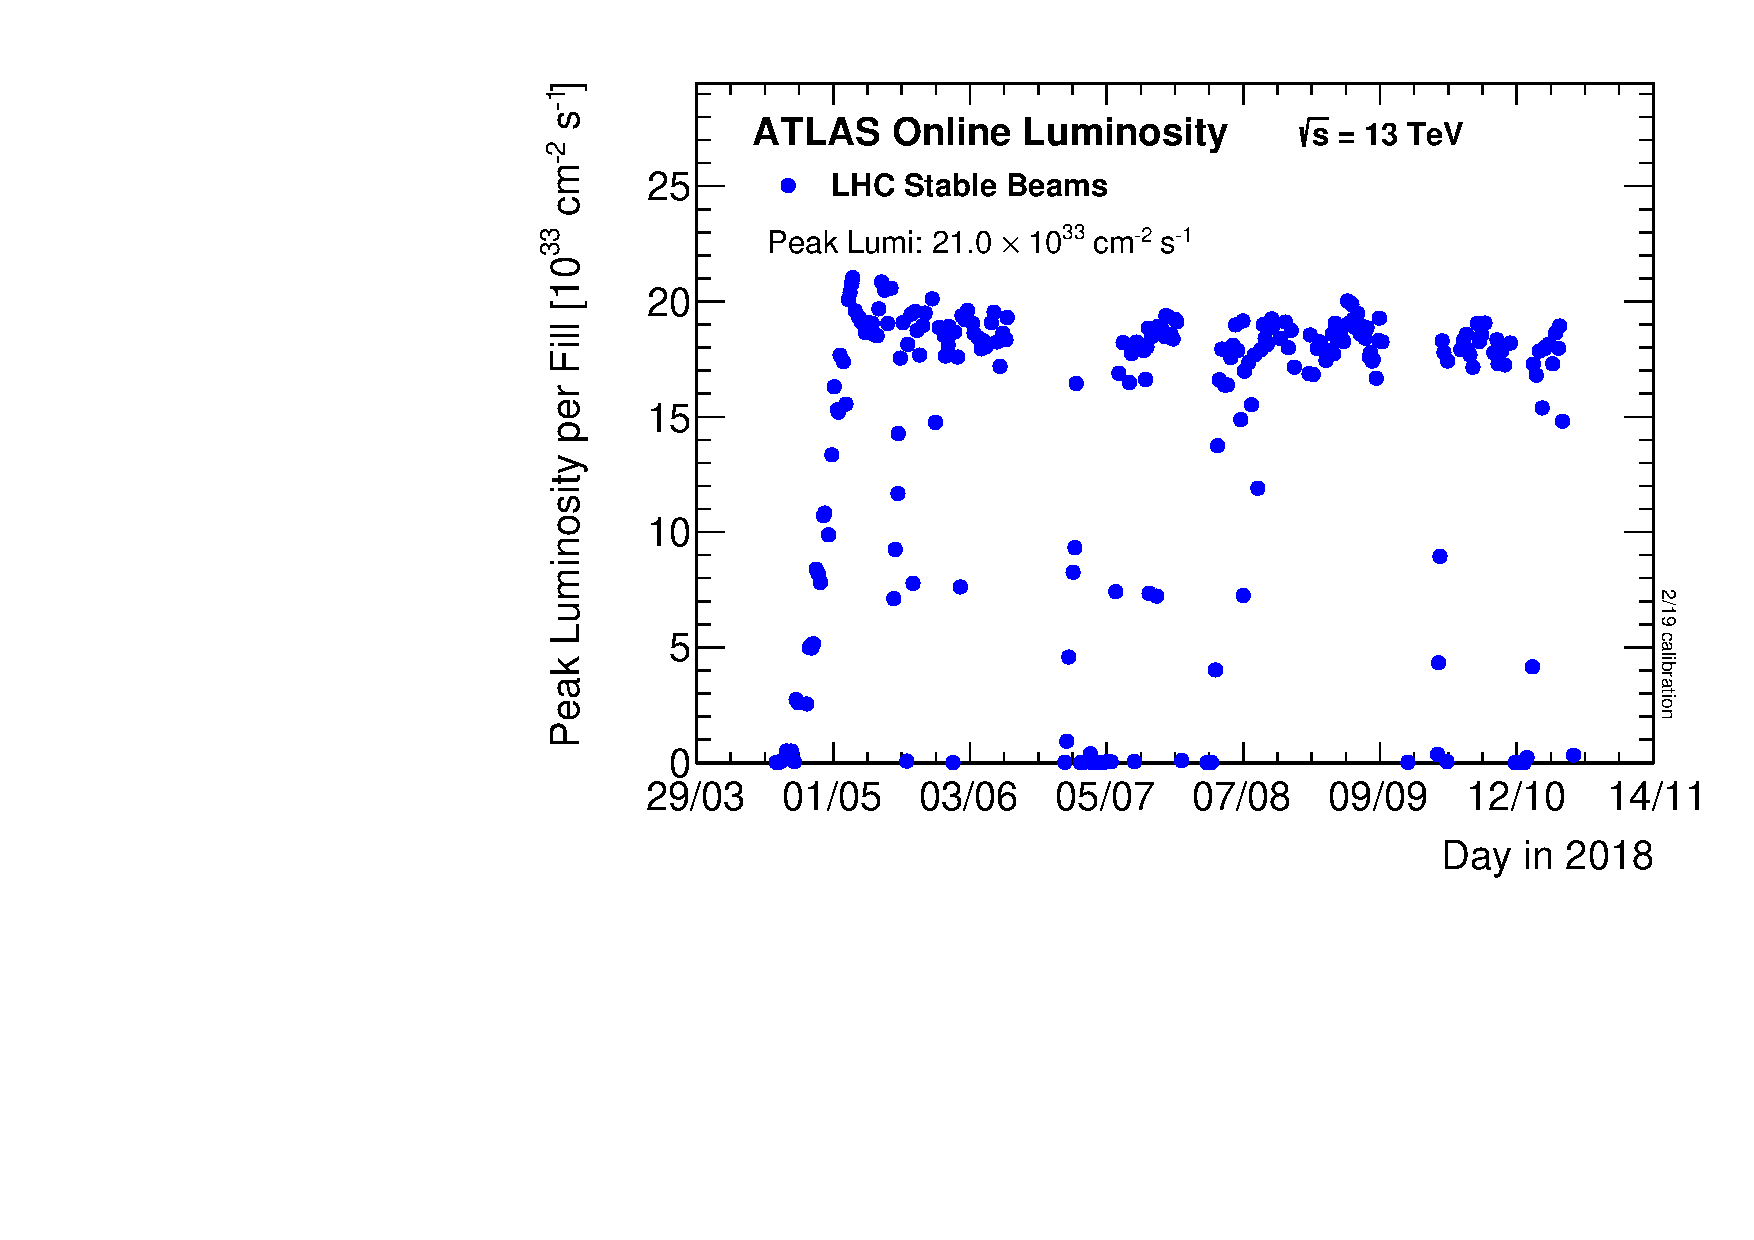
\includegraphics[width=\textwidth]{peakLumiByFill}
		\caption{\label{fig:peakLumiByFill}}
	\end{subfigure}%
	\begin{subfigure}[b]{0.45\linewidth}
		\centering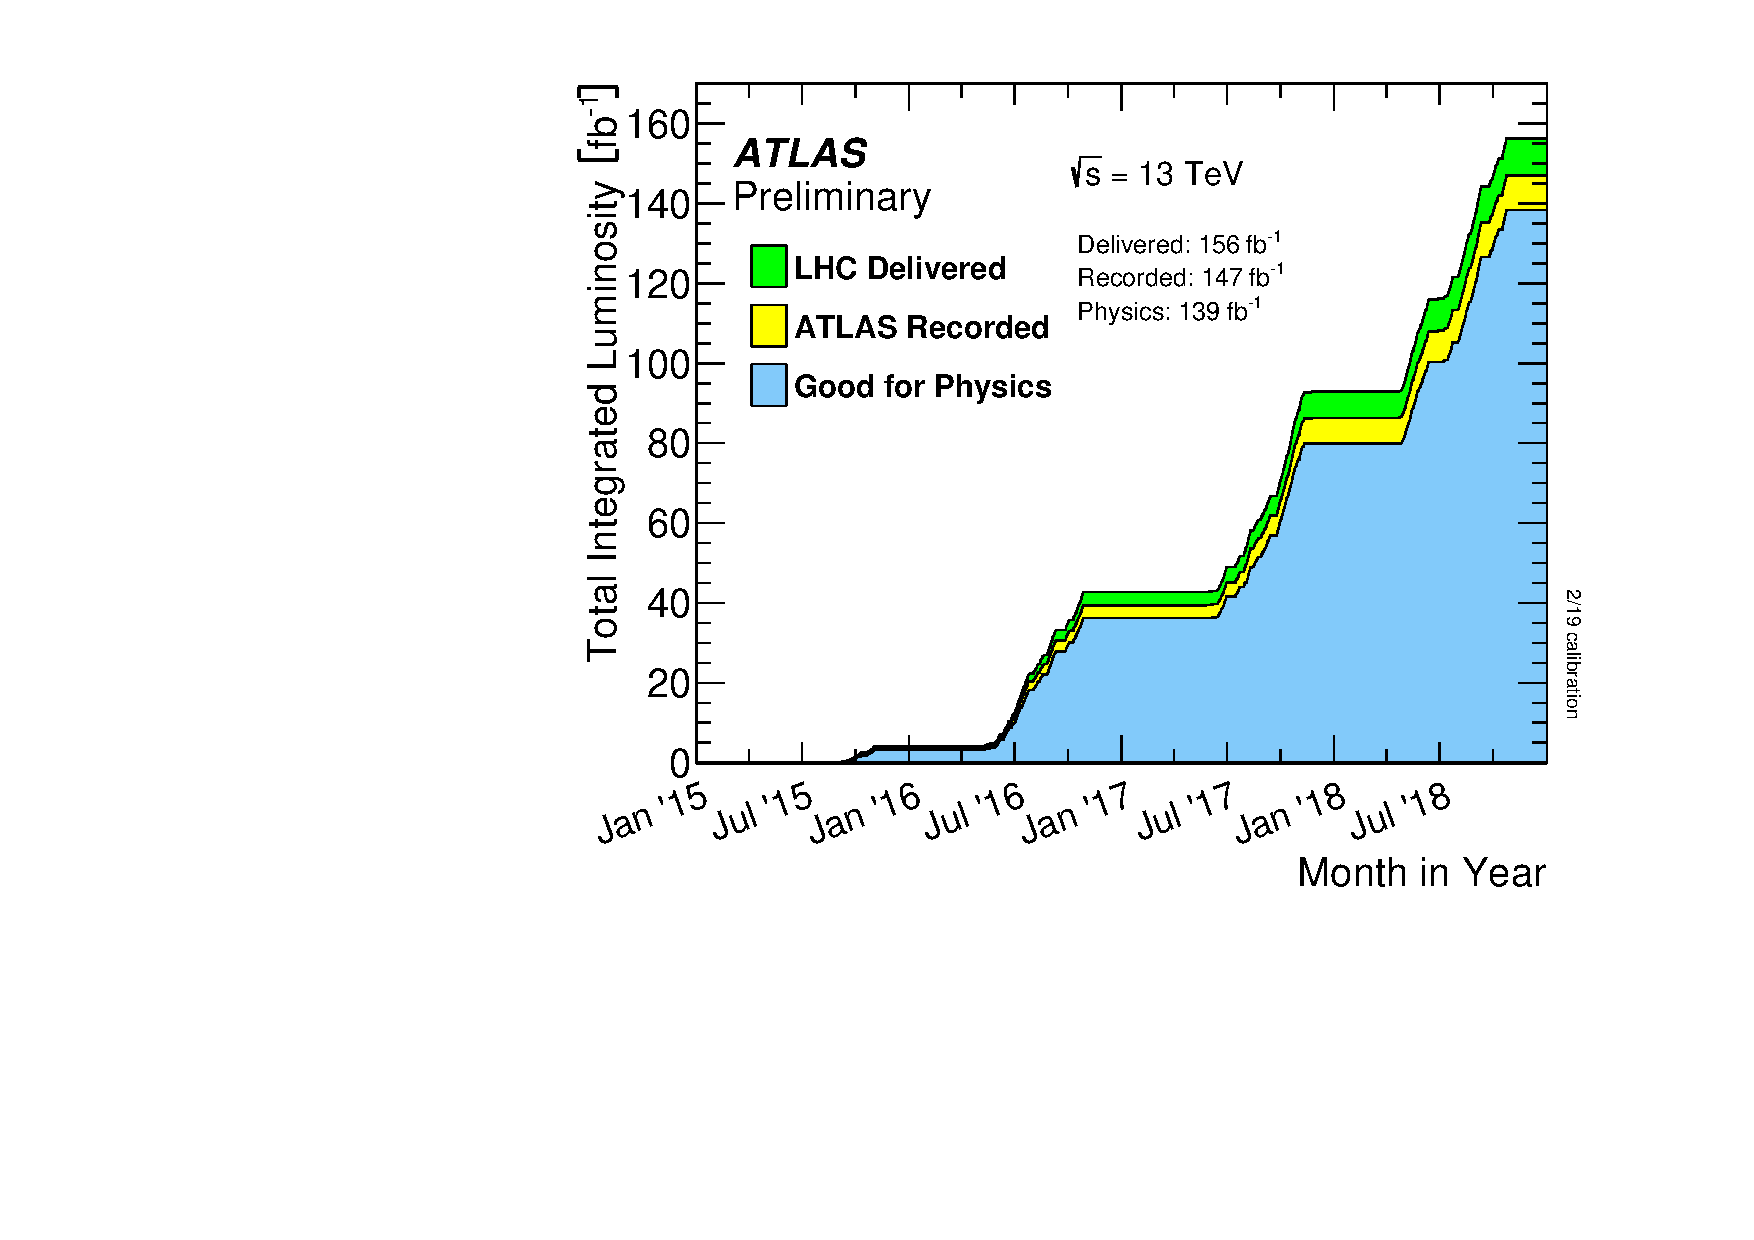
\includegraphics[width=\textwidth]{intlumivstimeRun2DQall}
		\caption{\label{fig:intlumivstimeRun2DQall}}
	\end{subfigure}%
	\caption{Instantaneous and cumulative luminosities in Run~2. Figure~\subref{fig:peakLumiByFill} shows the peak instantaneous luminosity delivered to ATLAS during $pp$ collision data taking in 2018 as a function of time. Figure~\subref{fig:intlumivstimeRun2DQall} shows the cumulative luminosity delivered to ATLAS (green), recorded by ATLAS (yellow) and deemed good for physics analysis (blue) during the entirety of Run~2~\cite{ATLAS:Run2}.}\label{fig:lumi_run2}
\end{figure}

Apart from the beam energy, the most important quantity for a collider is the instantaneous luminosity $L$. For a synchrotron with Gaussian beam distribution, the instantaneous luminosity can be written as
\begin{equation}
	L = \frac{N_b^2 n_b f_\mathrm{rev}}{4\pi\sigma_x\sigma_y} F,
	\label{eq:lumi}
\end{equation}
where $n_b$ is the number of bunches, $N_b$ the number of protons per bunch, $f_\mathrm{rev}$ the revolution frequency and $\sigma_x$ and $\sigma_y$ the transverse beam sizes. The parameters $F$ is a geometrical correction factor accounting for the reduction in instantaneous luminosity due to the beams crossing at a certain crossing angle. While the design instantaneous luminosity of the \gls{lhc} at the high-luminosity experiments ATLAS and CMS is $L = \SI{e34}{\per\cm\squared\per\second}$~\cite{Evans:1129806}, the 2017 and 2018 data-taking periods saw a peak luminosity twice as high~\cite{peak_lumi}.

The instantaneous luminosity is related to the total number of events $N$ through the cross section $\sigma$ of the events in question
\begin{equation}
	N = \sigma L_\mathrm{int} = \sigma \int L\diff t,
\end{equation}
with $L_\mathrm{int}$ the total integrated luminosity, a measure for the total amount of collision data produced.

A precise knowledge of the integrated luminosity corresponding to a given dataset is crucial for both SM measurements as well as searches for \gls{bsm} physics. Searches for \gls{susy} like the one presented in this work rely on precise measurements of the integrated luminosity in order to be able to estimate the contribution from SM background processes. The luminosity measurement for the Run~2 dataset used within this work is described in detail in~\cite{ATLAS-CONF-2019-021,Aaboud:2016hhf} and relies on a measurement of the bunch luminosity, \ie the luminosity produced by a single pair of colliding bunches
\begin{equation}
	L_b = \frac{\mu f_\mathrm{rev}}{	\sigma_\mathrm{inel}} = \frac{\mu_\mathrm{vis}f_\mathrm{rev}}{\sigma_\mathrm{vis}},
\end{equation}
with $\mu$ the pile-up parameter, $\sigma_\mathrm{inel}$ the cross section of inelastic $pp$ collisions, $\mu_\mathrm{vis} = \epsilon \mu$ is the fraction $\epsilon$ of the pile-up parameter $\mu$ visible to the detector and $\sigma_\mathrm{vis} = \epsilon\sigma_\mathrm{inel}$ the visible inelastic cross section. If $\sigma_\mathrm{vis}$ is known, the currently recorded luminosity can be determined by measuring $\mu_\mathrm{vis}$. At the ATLAS experiment, the observed number of inelastic interactions per bunch crossing $\mu\mathrm{vis}$ is measured using dedicated detectors, as for example LUCID-2~\cite{Avoni_2018}, a forward Cherenkov-detector using the quartz windows from photomultipliers as Cherenkov medium.
In order to use $\mu_\mathrm{vis}$ as luminosity monitor, the respective detectors need to be calibrated through a measurement of the visible inelastic cross section $\sigma_\mathrm{vis}$. This can be done using \gls{vdm} scans~\cite{vanderMeer:296752,GRAFSTROM201597}, in which the transverse distribution of protons in the bunches is inferred by measuring the relative interaction rates as a function of the transverse beam separation\footnote{Often called \textit{beam sweeping}.}. The algorithms used to determine the $\sigma_\mathrm{vis}$ calibration are described in~\cite{ATLAS-CONF-2019-021,Aaboud:2016hhf} and the luminosity during the \gls{vdm} runs can be determined using~\cref{eq:lumi}. At the \gls{lhc}, \gls{vdm} scans are typically performed in special low-$\mu$ runs with well-known machine parameters in order to minimise uncertainties~\cite{ATLAS-CONF-2019-021}. During high-$\mu$ physics runs, the luminosity measurement is then an extrapolation from the \gls{vdm} runs.

The \gls{lhc} entered operation in 2008, with first beams in September and first collisions by the end of November that same year~\cite{startup}. Its operation is in general structured into so-called \textit{Runs}, that are spanned by multiple years of data-taking. Run~1 spanned from 2009 to 2013 and delivered roughly $\SI{28.5}{\per\femto\barn}$ of $pp$ collision data to ATLAS, taken at centre-of-mass energies of $\SI{7}{\TeV}$ and $\SI{8}{\TeV}$~\cite{Aad:2011dr,Aad:1517411,Aaboud:2016hhf}. Run~2 lasted from 2015 to 2018 and saw a centre-of-mass energy increase to $\SI{13}{\TeV}$, delivering approximately $\SI{156}{\per\femto\barn}$ of $pp$ collision data to ATLAS~\cite{ATLAS-CONF-2019-021}. Run~3 of $pp$ collision data taking with two times design peak luminosity is currently planned to start its physics program in 2022 and last until end of 2024~\cite{run3}. Current plans foresee Run~3 to deliver about $\SI{150}{\per\femto\barn}$ of $pp$ collision data with centre-of-mass energies of $\SI{13}{\TeV}$ and $\SI{14}{\TeV}$. After Run~3, the \gls{lhc} will be upgraded to the High Luminosity \gls{lhc}, significantly increasing the peak instantaneous luminosity and delivering up to $\SI{3000}{\per\femto\barn}$ of $pp$ collision data from 2027 until 2040~\cite{run3,Apollinari:2284929}. 

This work uses $pp$ collision data taken by ATLAS during Run~2 of the \gls{lhc}. Of the $\SI{156}{\per\femto\barn}$ delivered to ATLAS, $\SI{147}{\per\femto\barn}$ were recorded, and $\SI{139}{\per\femto\barn}$ were deemed to be good for physics analysis. \Cref{fig:lumi_run2} shows the cumulative luminosity delivered to ATLAS during Run~2. Uncertainties on the measurement total recorded luminosity stem from the measurements of $\mu_\mathrm{vis}$ and $\sigma_\mathrm{vis}$, but are dominated by the uncertainties on $\sigma_\mathrm{vis}$ as \gls{vdm} scans can only be done during special runs, while the general conditions during high-$\mu$ conditions change continuously. For the full Run~2 dataset, the uncertainties accumulate to $\pm 1.7 \%$~\cite{ATLAS-CONF-2019-021}.

\section{ATLAS Experiment}\label{sec:atlas_experiment}

The ATLAS experiment is one of two general-purpose detectors at the LHC. Located at Point~1 in a cavern $\SI{100}{\meter}$ below the surface, it is approximately $\SI{44}{\meter}$ long and $\SI{25}{\meter}$ high~\cite{Aad:2008zzm}. The design of the ATLAS experiment is driven by the aim to allow for a diverse research program, including SM precision measurements, Higgs physics and searches for \gls{bsm} physics, whilst at the same time taking into account the unique and challenging conditions set by the \gls{lhc}. The various detector technologies used are designed to withstand the high-radiation environment of the \gls{lhc}, while allowing particle measurements with high spatial and temporal granularity. The general structure of ATLAS is depicted in \cref{fig:atlas_detector}, and consists of a central part, called \textit{barrel}, that has a cylindrical shape around the beam pipe, and two discs, called \textit{end-caps}, that close off the barrel on each side. This makes the ATLAS detector forward-backward symmetric and covering nearly the full solid angle of $4\pi$, which is needed in order to measure momentum imbalances caused by particles that only interact weakly with the detector material.

The interface between the ATLAS experiment and the \gls{lhc} is the beam pipe. In order to be maximally transparent to the particles created in the collisions, but also be able to withstand the forces from the vacuum, the beam pipe is made out of Beryllium close to the \gls{ip}, and stainless-steel further away from the \gls{ip}~\cite{Brock:1354959}.

The following sections introduce the working principles of the different detector components used in ATLAS, starting with the innermost component closest to the \gls{ip}, the inner detector, followed by the calorimeters in the middle and finally the muon spectrometers on the outside. If not otherwise stated, details on the detector components are extracted from~\cite{Aad:2008zzm}.

\begin{figure}
	\centering    
	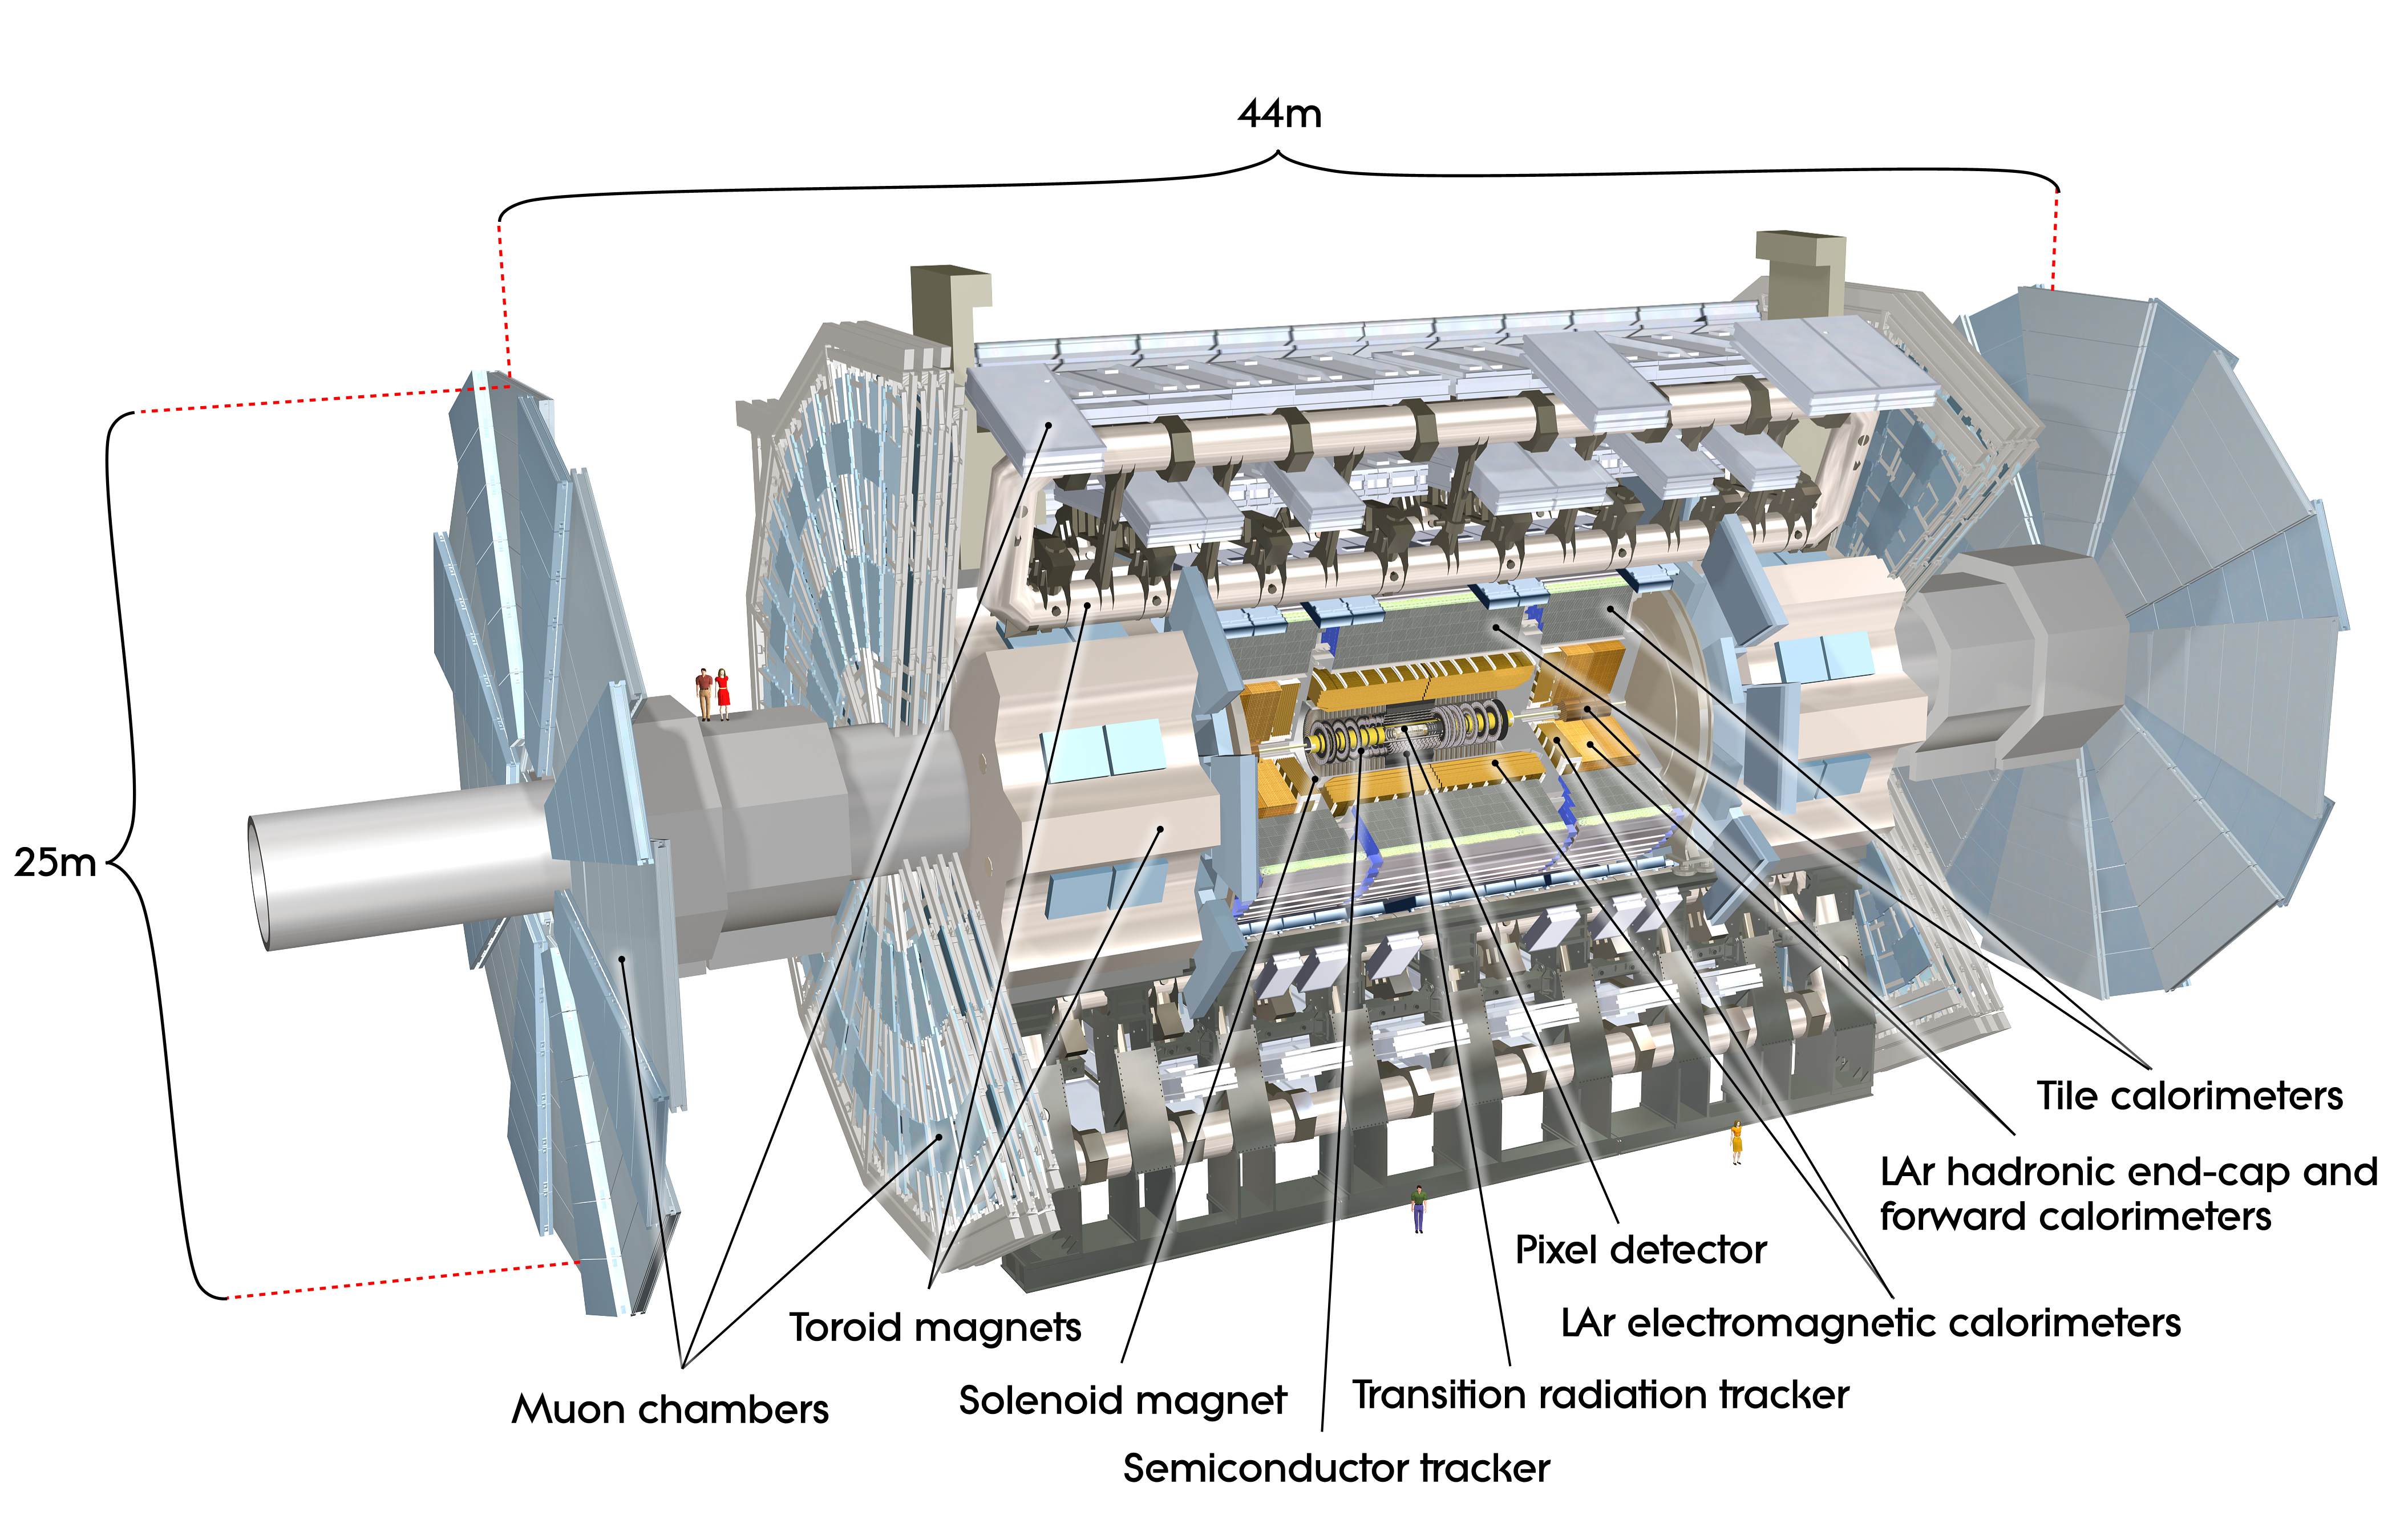
\includegraphics[width=0.9\textwidth]{atlas}
	\caption[The ATLAS detector]{Computer generated picture of the ATLAS detector, giving an overview on the various subsystems~\cite{Pequenao:1095924}.}
	\label{fig:atlas_detector}
\end{figure}


\subsection{Coordinate system}

In order to properly describe collision events in the ATLAS detector, a suitable detector system is needed. The right-handed coordinate system~\cite{ATLAS:1999uwa} used in ATLAS has its origin at the nominal \gls{ip} in the centre of the detector. The positive $x$-axis points towards the centre of the \gls{lhc} ring, the positive $y$-axis points upwards to the surface, and the beam pipe is used to define the $z$-axis. In the $x$--$y$ plane, called the transverse plane, the azimuthal angle $\phi$ is the angle around the beam axis, and the polar angle $\theta$ is measured from the beam axis. The rapidity~\cite{pdg2020} is defined as
\begin{equation}
	y = \frac{1}{2}\ln\left(\frac{E+p_z}{E-p_z}\right) = \tanh{\frac{p_z}{E}}^{-1},
\end{equation}
with $E$ the energy of an object and $p_z$ its momentum in $z$-direction. As opposed to the polar angle $\theta$, differences in the rapidity are invariant under Lorentz boosts in $z$-direction.

The pseudorapidity \cite{pdg2020} is the high-energy limit ($p\gg m$) of the rapidity, and defined as
\begin{align}
	\eta = - \ln\tan\frac{\theta}{2},
\end{align}
with $\cos\theta = p_z/p$. Pseudorapidity and rapidity are approximately equal in the limit where $p\gg m$ and $\theta \gg \frac{1}{\gamma}$. Compared to the rapidity, the pseudorapidity has the advantage of not depending on the energy and momentum calibration of the detected objects. Additionally, it gives a direct correspondence to the polar angle $\theta$ through the relation $\tanh\eta = \cos\theta$. Objects travelling along the beam axis have a pseudorapidity of $\eta = \inf$ and objects travelling upwards along the $y$-axis have $\eta = 0$.

The distance between two objects in the ATLAS detector is given by
\begin{align}
	\Delta R=\sqrt{\left(\Delta \eta\right)^2+\left(\Delta \phi\right)^2}.
\end{align}
The longitudinal momentum of the partons composing the colliding hadrons is only known by means of the \glspl{PDF}, giving the probabilities of the partons to have a certain energy in the direction of the beam. Thus, the total longitudinal energy in each collision is not exactly known, impeding the use of physics quantities in the $z$-direction. In the $x$--$y$ plane, however, momentum conservation can be applied, which is why mainly transverse physics quantities are used, indicated by a subscript `T', \eg $E_T$ or $p_T$.

\subsection{Magnet system}

In order to perform precise momentum measurements of particles, ATLAS uses a system of magnets, whose magnetic fields force charged particles on curved tracks due to the Lorentz force. Using precise measurements of the tracks taken in the inner detector and the muon spectrometers, the curvature of the tracks can be determined, allowing an inference of the charge-to-momentum ratio $q/p$ of charged particles. ATLAS employs a set of four superconducting magnets, one central solenoid, and three toroids, all operating at a nominal temperature of $\SI{4.5}{K}$, achieved through a cryogenic system using liquid helium~\cite{Aad:2008zzm}. 

The solenoid is aligned on the beam axis and provides a $\SI{2}{T}$ magnetic field for the inner detector~\cite{Aad:2008zzm}. As it is located in front of the calorimeters (as seen from the \gls{ip}), it is specially designed to have minimal material thickness in order to avoid influencing the subsequent energy measurements. The solenoid consists of single-layer coils made out of a Nb/Ti conductor and additional aluminum for stability. It operates at a nominal current of $\SI{7.73}{\kilo\ampere}$ and uses the hadronic calorimeter as return yoke~\cite{Aad:2008zzm}.

The toroid magnets consist of a barrel toroid and two end-cap toroids, producing a magnetic field of $\SI{0.5}{T}$ and $\SI{1}{T}$ for the muon spectrometers in the barrel and end-caps, respectively\footnote{The magnetic field in of the toroid magnets is designed to be higher in the end-caps in order to ensure enough bending power necessary for precise momentum measurements.}~\cite{Aad:2008zzm}. Both barrel and end-cap toroids are made out off Nb/Ti/Cu conductor with aluminum stabilisation, wound into double pancake-shaped coils. The barrel toroid coils are enclosed in eight stainless-steel vacuum vessels in a racetrack-shaped configuration and arranged around the barrel calorimeters with an azimuthal symmetry. In order to withstand the Lorentz forces, the end-cap toroid coils are assembled in eight square units, and bolted and glued together with eight wedges, forming rigid structures. Both end-cap and barrel toroids operate at a nominal current of $\SI{20.5}{\kilo\ampere}$~\cite{Aad:2008zzm}.

\subsection{Inner detector}

Embedded in the magnetic field of the solenoid, the \gls{id} measures tracks of charged particles, allowing a determination of their momentum, while also providing crucial information for vertex reconstruction. As the \gls{id} is the detector closest to the beam pipe, its components need to be able to withstand the extreme high-radiation environment close to the \gls{ip}. The \gls{id} consists of three subdetectors and uses two different working principles: semiconductor and gaseous detectors. In semiconductor-based tracking detectors, charged particles passing through the detector create a trail of electron-hole pairs that subsequently drift through the semiconductor material and cause electric signals. In gaseous detectors, traversing particles create electron-ion pairs also drift towards metal electrodes and induce electric signals.

 Closest to the \gls{id} lies the pixel detector, followed by the \gls{sct}, both of which are made of semiconductors. The \gls{sct} is surrounded by the \gls{trt}, a gaseous detector. In total, the \gls{id} provides tracking and momentum information within $\vert\eta\vert < 2.5$ and down to transverse momenta of nominally $\SI{0.5}{\GeV}$. A schematic illustration of the \gls{id} and its subdetectors is shown in \cref{fig:ID_schematic}. 

\begin{figure}
	\centering
	\begin{subfigure}[b]{0.45\linewidth}
		\centering\includegraphics[width=\textwidth]{id}
	\end{subfigure}%
	\begin{subfigure}[b]{0.45\linewidth}
		\centering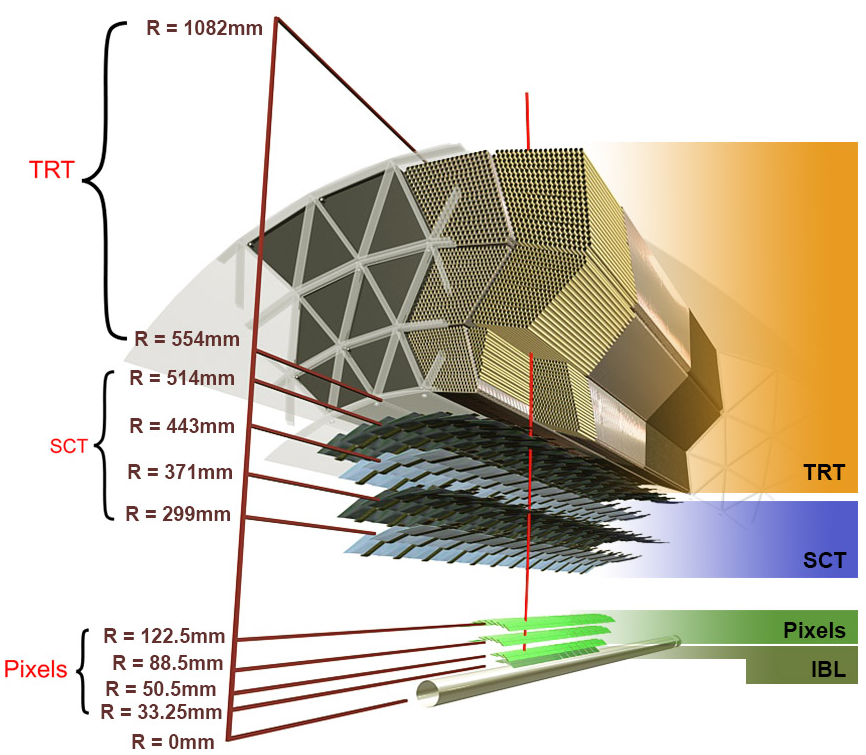
\includegraphics[width=\textwidth]{ibl}
	\end{subfigure}%
	\caption{Schematic drawing of the ID and its subdetectors. Images adapted from~\cite{Pequenao:1095926, Potamianos:2209070}.}\label{fig:ID_schematic}
\end{figure}

\subsubsection{Pixel detector}

In the high-rate environment directly adjacent to the beam pipe, the only detector technology able to operate and deliver high-precision tracking information are semiconductor detectors segmented into pixels. As opposed to strip detectors, the reduced size of silicon pixel detectors and thus significantly reduced hit rate per readout channel allows pixel detectors to still be operational in the harsh environment close to the IP. In ATLAS, pixels are hybrids of sensors and readout electronics, and were originally arranged in three layers in the barrel and the end-caps with a typical pixel of $\SI{50}{\micro\meter}\times \SI{400}{\micro\meter}$, covering pseudorapidities up to $\vert\eta\vert < 2.5$. In order to increase robustness  and performance in the high-luminosity environment, a new innermost layer, called the \gls{ibl}, was installed together with a new, smaller radius beam pipe between Run~1 and Run~2~\cite{Abbott:2018ikt,Capeans:1291633}. The IBL uses smaller pixels with a size of $\SI{50}{\micro\meter}\times \SI{250}{\micro\meter}$ and improves the tracking precision as well as vertex identification performance~\cite{Capeans:1291633}. It also improves the performance of identifying jets originating from $b$-quarks (called \textit{b}-tagging). The pixel detector~\cite{Aad:2019aic}. The tracking precision obtained by the pixel detector is $\SI{10}{\micro\meter}$ in ($R-\phi$) and $\SI{115}{\micro\meter}$ in ($z$) for the barrel and ($R$) for the end-caps.

\subsubsection{Silicon microstrip detector}

The pixel detector is surrounded by the \gls{sct}, consisting of four layers in the barrel and nine disks in the end-caps. In order to provide two-dimensional tracking information, strips are arranged in double-layers with a small crossing angle of $\SI{40}{mrad}$ and a mean pitch of $\SI{80}{\micro\meter}$~\cite{Aad:2008zzm}. A charged particle traversing the \gls{sct} through the barrel thus creates four space point measurements. In the barrel, one set of strips in each of the four double-layers is oriented in beam direction, thereby measuring $R-\phi$, and in the end-caps, one set of strips in each layer is oriented in radial direction. The \gls{sct} has roughly $6.3$ million readout channels and provides tracking information up to $\vert\eta\vert <2.5$~\cite{Aad:2008zzm}. It achieves a precision of $\SI{17}{\micro\meter}$ in ($R-\phi$) and $\SI{580}{\micro\meter}$ in ($z$) for the barrel and ($R$) for the end-caps~\cite{Aad:2008zzm}.

\subsubsection{Transition radiation tracker}

The last and also largest of the three subdetectors of the \gls{id} is the \gls{trt}, a gaseous detector made of multiple layers of $\SI{4}{\milli\meter}$ diameter drift tubes, surrounding the pixel detector and the \gls{sct}. The drift tubes consist of an aluminum cathode coated on a polyimide layer reinforced by carbon fibers and use a gold-plated tungsten wire as anode. The tubes are filled with a Xe-based gas mixture, providing an electric permittivity different from the surrounding material, causing transition radiation when traversed by ultrarelativistic particles. While the $\SI{144}{\centi\meter}$ long tubes in the barrel region are aligned parallel to the beam pipe, the $\SI{37}{\centi\meter}$ long tubes in the end-caps are aligned in radial direction, providing coverage up to $\vert\eta\vert <2.0$ and an intrinsic accuracy of $\SI{130}{\micro\meter}$ in $R-\phi$~\cite{Aad:2008zzm}. The low accuracy compared to the pixel detector and the \gls{sct} is compensated by the large amount of hits (typically $36$ per track) and the longer measured track length. As the amount of transition radiation given off by a particle, is proportional to its Lorentz factor $\gamma$~\cite{pdg2020}, the \gls{trt} is also used to improve electron identification~\cite{ATLAS-CONF-2011-128}. For the same momentum, electrons will have a higher Lorentz factor than the heavier charged pions, and consequently give off more transition radiation.

\subsection{Calorimeters}

\begin{figure}
	\centering
	\begin{subfigure}[b]{0.45\linewidth}
		\centering\includegraphics[width=\textwidth]{cal}
		\caption{Calorimeter systems\label{fig:calorimeters}}
	\end{subfigure}%
	\begin{subfigure}[b]{0.45\linewidth}
		\centering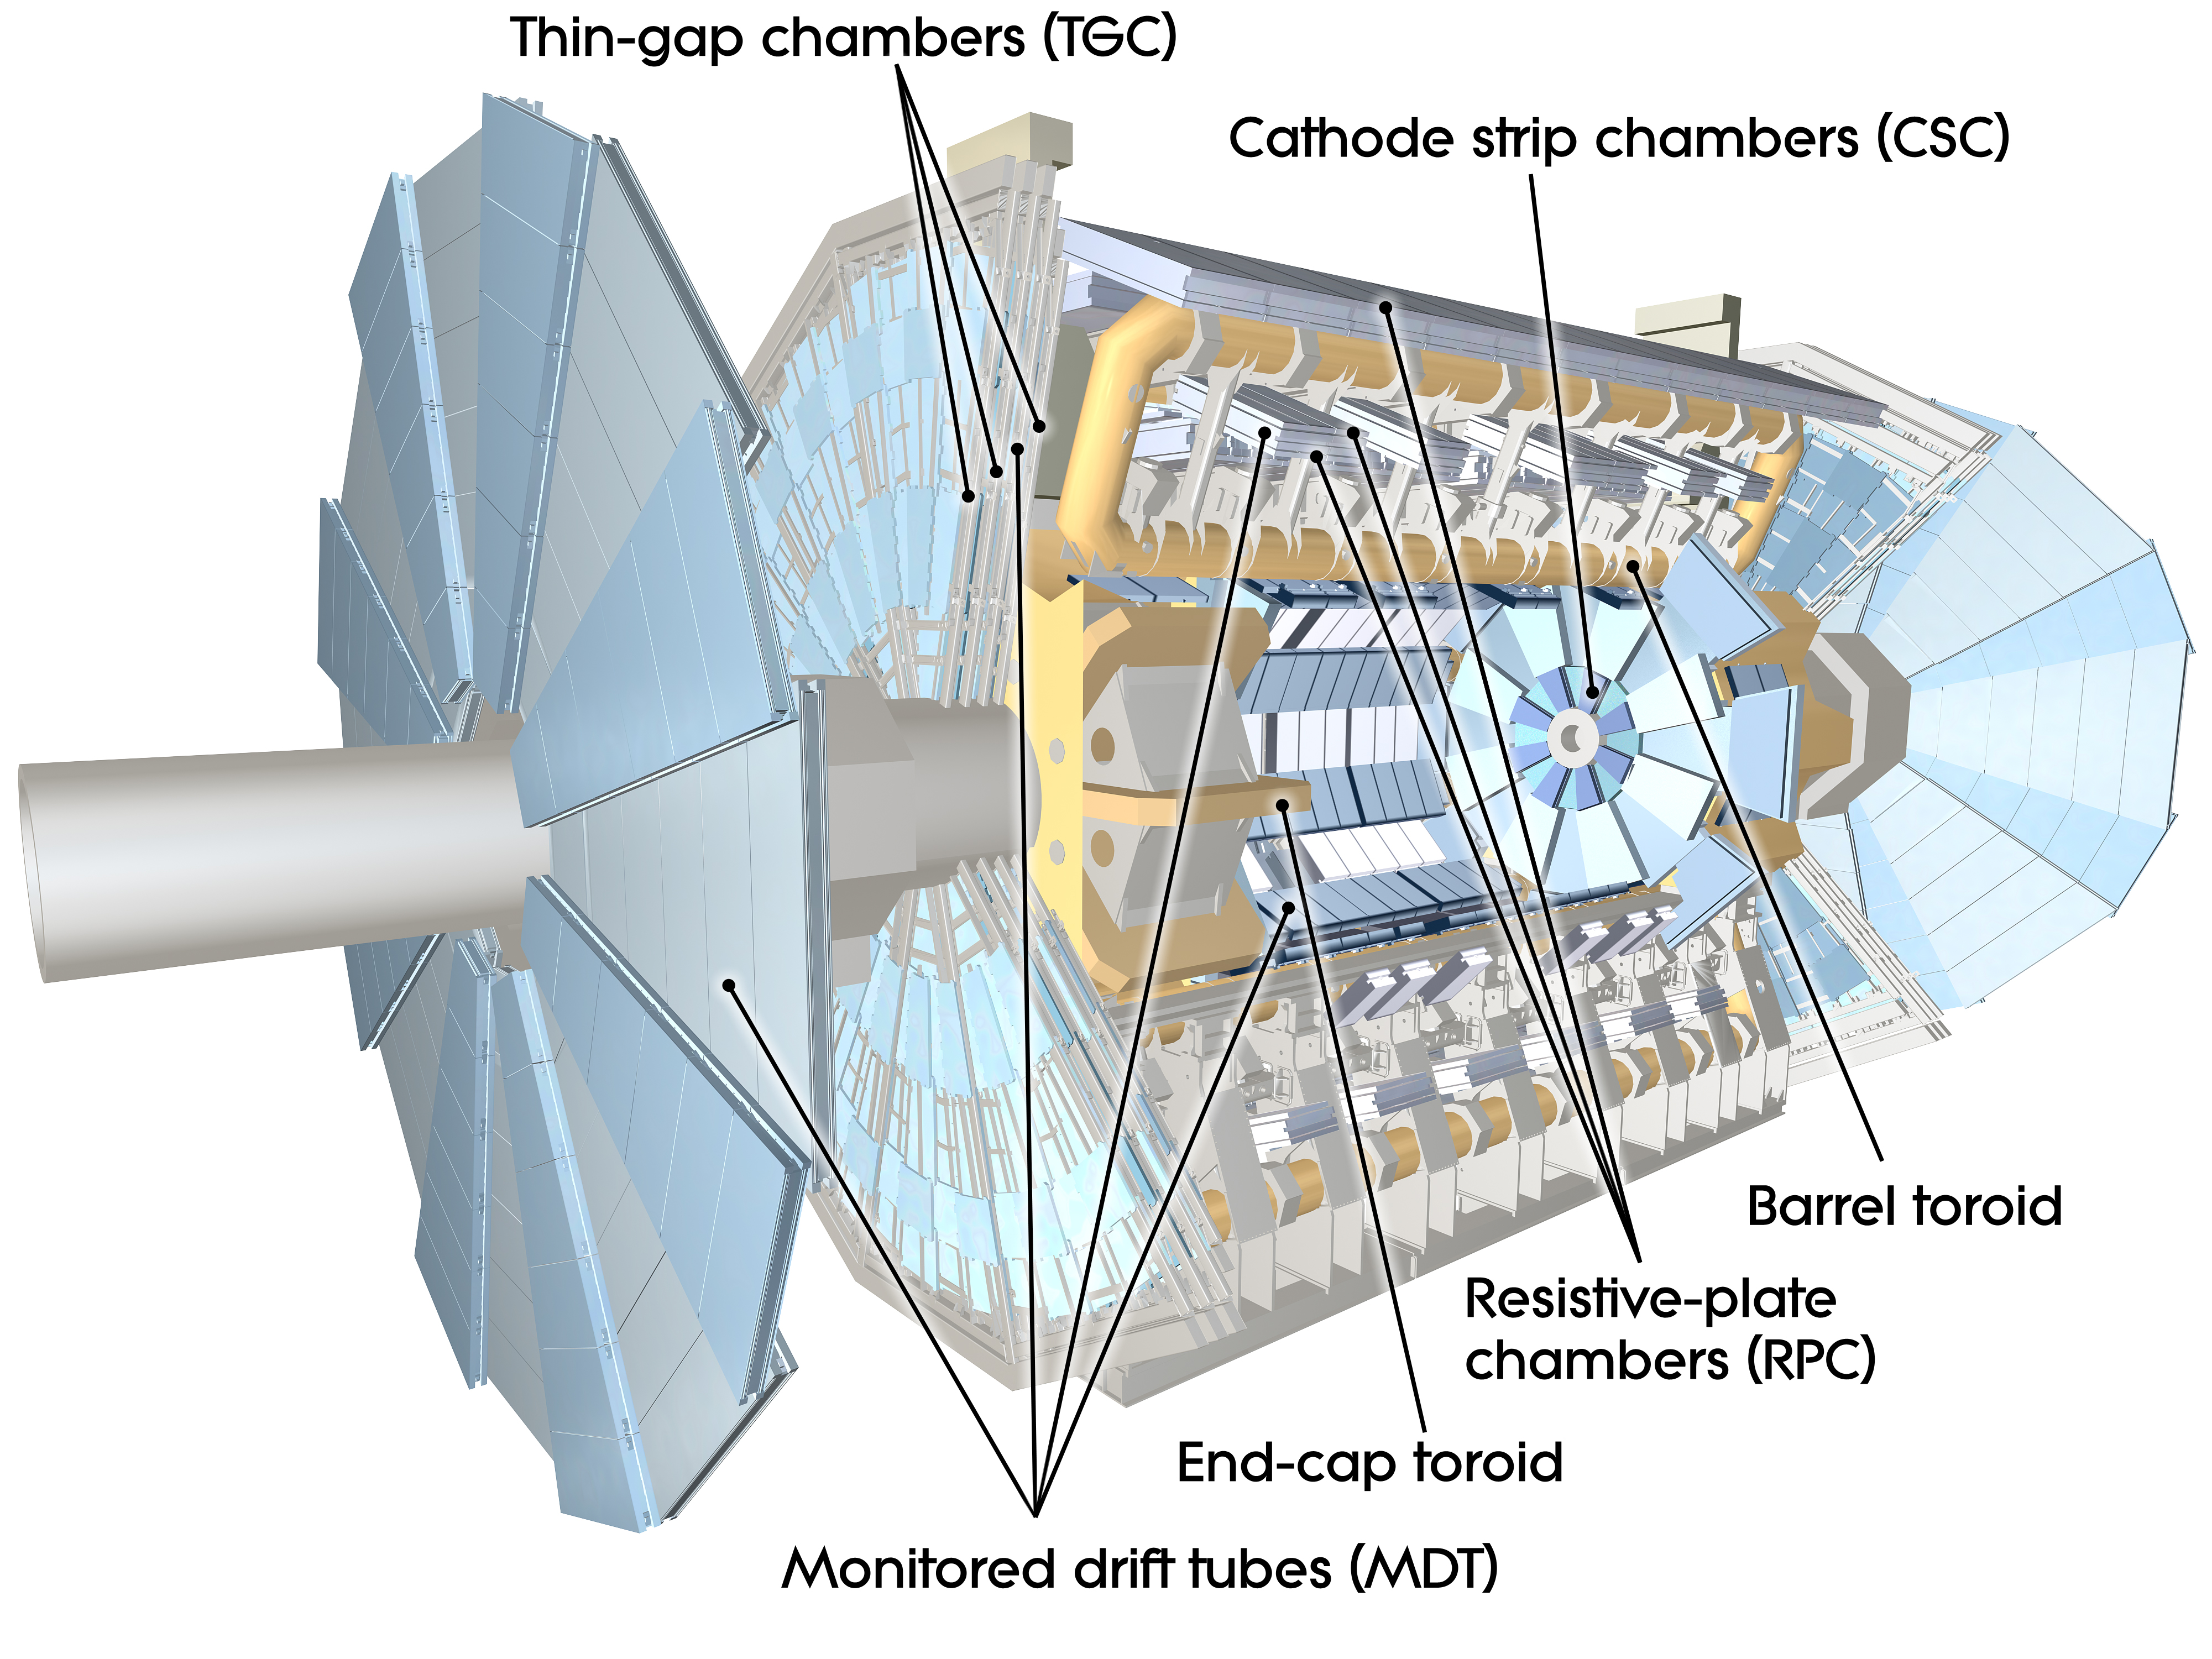
\includegraphics[width=\textwidth]{ms}
		\caption{Muon spectrometer\label{fig:muon_system}}
	\end{subfigure}%
	\caption{Schematic drawing of the calorimeter systems and the muon spectrometer in ATLAS. Images adapted from~\cite{Pequenao:1095927,Pequenao:1095929}.}\label{fig:cal_ms_schematic}
\end{figure}

The primary goal of calorimeters is to measure the energies of incoming particles by completely absorbing them. As the energies of neutral particles can not be measured by other means, calorimeters are especially important for jet energy measurements (which contain neutral hadrons)~\cite{Brock:1354959}. Since particles like photons and electrons interact mostly electromagnetically, while hadrons predominantly interact through the strong interaction, two different calorimeter types are needed in ATLAS. For values in $\eta$ matching the \gls{id}, the electromagnetic calorimeter uses a finer granularity designed for precision measurements of electrons and photons. The subsequent hadronic calorimeter uses a coarser granularity sufficient for the requirements of jet reconstruction and missing transverse moment measurements. With a coverage up to $\vert\eta\vert <4.9$, the calorimeter system in ATLAS provides the near hermetic energy measurements needed for the inference of missing transverse momentum created by neutrinos and other weakly interacting neutral particles~\cite{Aad:2008zzm}.

Both calorimeters are sampling calorimeters, consisting of alternating layers of active and absorbing material. The absorbing material interacts with the incoming particles, causing them to deposit their energy by creating cascades or \textit{showers} of secondary particles. The active layers are then used to record the shape and intensity of the produced showers. This alternating structure results in reduced material costs but also reduced energy resolution as only part of the particle's energy is sampled. Due to the typically longer cascades in hadronic interactions compared to electromagnetic interactions, and in order to minimise punch-through into the muon system, the hadronic calorimeter requires a greater material depth than the electromagnetic one. The calorimeter systems in ATLAS are schematically illustrated in \cref{fig:calorimeters}.

\subsubsection{Electromagnetic calorimeter}

The \gls{em} calorimeter has an accordion-shaped structure and uses \gls{lar} as active material and lead as absorber, providing full $\phi$ symmetry without azimuthal cracks. It is divided into a barrel part and two end-caps, covering $\vert\eta\vert <1.475$ and $1.375 < \vert\eta\vert <3.2$, respectively, and arranged in a way to provide uniform performance and resolution as a function of $\phi$. The barrel \gls{em} calorimeter consists of two identical half-barrels with a small gap of $\SI{4}{\centi\meter}$ at $z=0$. In the end-caps, the \gls{em} calorimeter consists of two coaxial wheels, covering the region $1.375 < \vert\eta\vert <2.5$ and $2.5 < \vert\eta\vert <3.2$, respectively. Calorimeter cells in the \gls{em} calorimeter are segmented into multiple layers with fine granularity in first layers in the $\eta$ region matching the ID, and coarser granularity in the outer layers and for $2.5 < \vert\eta\vert <3.2$. In order to offer good containment of electromagnetic showers, the \gls{em} calorimeter has a depth of at least $22$ ($24$) radiation lengths in the barrel (end-caps). A single instrumented \gls{lar} layer serves as presampler in the region with $\vert\eta\vert <1.8$, allowing measurements of the energy losses upstream of the \gls{em} calorimeter, \eg in the cryostats~\cite{Aad:2008zzm}. The design energy resolution of the \gls{em} calorimeter is $\sigma_E / E = 10\% / \sqrt{E} \oplus 0.7\%$~\cite{Aad:2008zzm}.

\subsubsection{Hadronic calorimeter}

Placed directly outside the envelope of the \gls{em} calorimeter is the hadronic tile calorimeter. It uses steel plates as absorber and polystyrene-based scintillating tiles as active material, and is subdivided into one central barrel and two extended barrels. Each barrel is segmented in three layers in depth with a total thickness of $7.4$ interaction lengths. The tiles are oriented radially and perpendicular to the beam pipe and grouped in 64 tile modules per barrel, resulting in a near hermetic azimuthal coverage. Wavelength shifting fibres are used to shift the ultraviolet light produced in the scintillator to visible light and guide it into photomultipliers located at the radially far end of each module. The tile calorimeter covers a region with $\vert\eta\vert <1.7$ and has a granularity of $\Delta \eta \times \Delta \phi = 0.1 \times 0.1$ except for the outermost layer which has a slightly coarser granularity in $\eta$. The design energy resolution of the tile calorimeter is $\sigma_E / E = 56.4\% / \sqrt{E} \oplus 5.5\%$~\cite{Aad:2008zzm}.

Hadronic calorimetry in the end-caps is provided by two independent calorimeter wheels per end-cap, situated directly behind the \gls{emec}. Similar to the \gls{emec}, the \gls{hec} also uses \gls{lar} calorimeter as active material, allowing both calorimeter systems to share a single cryostat per end-cap. Instead of lead, the HEC however uses copper as absorber, which not only drastically reduces the mass of a calorimeter with a given interaction length, but also improves the linearity of low-energy hadronic signals~\cite{Lee:2637852}. Each of the four wheels of the \gls{hec} is comprised of 32 wedge-shaped modules, divided into two layers in depth. The \gls{hec} provides coverage in the region with $1.5 < \vert\eta\vert <3.2$, slightly overlapping with the tile calorimeter and thus reducing the drop in material density in the transition region. While the granularity in the precision region with $1.5 < \vert\eta\vert <2.5$ is the same as for the tile calorimeter, more forward regions with large $\vert\eta\vert$ have a granularity of $\Delta \eta \times \Delta \phi = 0.2 \times 0.2$~\cite{Aad:2008zzm}. The design resolution of the \gls{hec} is $\sigma_E / E = 70.6\% / \sqrt{E} \oplus 5.8\%$~\cite{Aad:2008zzm}.

The forward region with $3.1 < \vert\eta\vert <4.9$ is covered by the \gls{lar}~\gls{fcal}, which is integrated into the end-cap cryostats. This hermetic design not only minimises energy losses in cracks between the calorimeter systems, but also reduces the amount of background reaching the muon system in the outer shell of the ATLAS experiment. In order to limit the amount of neutrons reflected into the \gls{id}, the \gls{fcal} is recessed by about $\SI{1.2}{\meter}$ with respect to the \gls{em} calorimeter, motivating a high-density design due to space constraints. The \gls{fcal} in each end-cap consists of three layers with a total depth of 10 interaction lengths. While the first layer uses copper as absorber and is optimised for electromagnetic measurements, the remaining two layers are made of tungsten and cover hadronic interactions. The metals comprising each layer are arranged in a matrix structure with electrodes consisting of rods and tubes parallel to the beam pipe filling out regular channels. The small gaps ($\SI{0.25}{\milli\meter}$ in the first layer) between the rods and tubes of the electrodes are filled with \gls{lar} as active material.

\subsection{Muon spectrometer}

Muons, being minimum ionising particles, are the only charged particles that consistently pass through the entire detector including the calorimeter system. Providing one of the cleanest signatures for \gls{bsm} physics~\cite{Brock:1354959}, muonic final states are measured with a dedicated detector system on the outermost layer of the ATLAS experiment. Embedded in the magnetic field of the toroid magnets, the \gls{ms} consists of three concentric cylindrical layers in the barrel region, and three wheels in each end-cap, and provides momentum measurements up to $\vert\eta\vert <2.7$~\cite{Aad:2008zzm}. It is designed to deliver a transverse momentum resolution of $10\%$ for $\SI{1}{\TeV}$ tracks and be able to measure muon momenta down to roughly $\SI{3}{\GeV}$.

The \gls{ms} uses two high-precision gaseous detector chamber types, \gls{mdt} chambers and \gls{csc}. As both the \gls{mdt} and \gls{csc} are drift chambers relying on charges drifting to an anode or cathode, the maximum response times of $\SI{700}{\nano\second}$ and $\SI{50}{\nano\second}$, respectively, are slow compared to the bunch-spacing of $\SI{25}{\nano\second}$. ATLAS therefore uses \gls{rpc} in the barrel and \gls{tgc} in the end-caps as triggers in order to associate measurements to the right bunch-crossing.  

\subsubsection{Monitored drift tubes}

The \gls{mdt} chambers are the main subcomponent providing precision measurements of the muon tracks up to $\vert\eta\vert <2.7$, except in the innermost end-cap layer where their coverage only extends to $\vert\eta\vert <2.0$. The \gls{mdt} are made of 3--4 layers of $\sim \SI{30}{\milli\meter}$ diameter drift tubes operated with Ar/CO$_2$ gas\footnote{With a small admixture of $\SI{300}{ppm}$ of water to improve high voltage stability.} pressurised to $\SI{3}{\bar}$. Charged particles traversing the drift tubes ionise the gas, creating electrons that drift towards a central tungsten-rhenium anode wire with a diameter of $\SI{50}{\micro\meter}$. Following the symmetry of the barrel toroid magnet, the \gls{mdt} chambers are arranged as octets around the calorimeters with the drift tubes in $\phi$ direction, \ie tangential to circles around the beam pipe. In order to be able to correct for potential chamber deformations due to varying thermal gradients, each \gls{mdt} chamber is equipped with an internal optical alignment system. Apart from the regular chambers in the barrel and the end-cap wheels, special modules are installed in order to minimise the acceptance losses due to the ATLAS support structure (the \textit{feets} of the experiment).

\subsubsection{Cathode strip chambers}

In the region with $\vert\eta\vert > 2.0$ in the first layer of the end-caps, the particle flux is too high to allow for safe operation of \gls{mdt} chambers. Instead, \gls{csc}, multiwire proportional chambers, are used for precision measurements in this region. The gold-plated tungsten-rhenium anode wires in the \gls{csc} have a diameter of $\SI{30}{\micro\meter}$ and are oriented in radial direction. The wires are enclosed on both sides by cathode planes, one segmented perpendicular to the wires (thus providing the precision coordinate), the other parallel to the wires. Each chambers is filled with an Ar/CO$_2$ gas mixture and consists of four wire planes, resulting in four measurements of $\eta$ and $\phi$ for each track. In addition to the chamber-internal alignment sensors, ATLAS also employs an optical alignment system in order to align the precision chambers to each other~\cite{Aad:2008zzm}.

\subsubsection{Resistive plate chambers}

\gls{rpc} are gaseous parallel electrode-plate chambers that use two resistive plastic laminate plates kept $\SI{2}{\milli\meter}$ apart by insulating spacers. Due to an electric field of roughly $\SI{4.9}{\kilo\volt\per\milli\meter}$ between the plates, charged particles traversing the chamber cause avalanches of charges that can be read out through capacitive coupling to metallic strips mounted on the outside of the resistive plates. In order to provide tracking information in both coordinates, each \gls{rpc} consists of two rectangular units each containing two gas volumes with a total of four pairwise orthogonal sets of readout strips. The tree concentric cylindrical layers of \gls{rpc} in the barrel region thus provide six measurements of $\eta$ and $\phi$ and cover $\vert\eta\vert <1.05$

\subsubsection{Thin gap chambers}

The \gls{tgc} are not only necessary for triggering in the end-cap \gls{ms} but also provide measurements of a second coordinate, orthogonal to the measurements of the \gls{mdt}. \gls{tgc} are multi-wire proportional chambers enclosed by two cathode planes and a wire-to-wire gap of $\SI{1.8}{\milli\meter}$. The gas mixture of CO$_2$ and n-pentane allows for a quasi-saturated operation mode resulting in a relatively low gas gain. Each \gls{tgc} unit is built from a doublet or triplet of such chambers, separated by a supporting honeycomb structure, In each unit, the azimuthal coordinate is measured by radial copper readout strips, while the bending coordinate is provided by the wire groups.The \gls{tgc} are mounted in two concentric disks in each end-cap, one covering the rapidity range $1.05 < \vert\eta\vert < 1.92$ and one covering the more forward region $1.92 < \vert\eta\vert <2.4$. 

\subsection{Forward detectors}

Apart from the relative luminosity monitor LUCID-2~\cite{Avoni_2018} (introduced in \cref{sec:lumi_datataking}) located at $\pm \SI{17}{\meter}$ from the \gls{ip}, ATLAS uses three additional small detectors in the forward region. At $\pm \SI{140}{\meter}$ from the \gls{ip}, immediately behind the location where the straight beam pipe splits back into two separate beam pipes, lies the \gls{zdc}~\cite{Leite:1628749}. The \gls{zdc} is embedded in an absorber for neutrals mainly measures forward neutrons with $\vert\eta\vert > 8.3$ in heavy-ion collisions. Even further out from the \gls{ip} at $\pm \SI{240}{\meter}$, lies the \gls{alfa} detector~\cite{AbdelKhalek:2016tiv}, consisting of scintillating fibre trackers placed in Roman pots~\cite{AMALDI1977390} measuring the absolute luminosity through small scattering angles of $\SI{3}{\micro\radian}$ (necessitating the special beam conditions also used for the LUCID-2 calibrations). The last of the forward detectors is the \gls{afp}~\cite{Adamczyk:2017378} detector, installed at the end of 2016 and operational since early 2017, is situated $\pm\SI{205}{\meter}$ and $\pm\SI{217}{\meter}$ from the \gls{ip} and consists of Roman pots containing silicon trackers and time-of-flight detectors. The \gls{afp} detectors aims to study very forward protons from elastic and diffractive scattering.

\subsection{Trigger and data acquisition system}

With a nominal bunch spacing of $\SI{25}{\nano\second}$, the bunch crossing rate within ATLAS is $\SI{40}{\MHz}$. Even with only a single $pp$ collision event per bunch crossing, a mean event size of $\sim \SI{1.6}{\mega\byte}$ results in a data volume of more than $\SI{60}{\tera\byte\per\second}$, which is impossible to process and write to disk with current technology. In addition, interesting physics events will often only occur at relatively low rates, and generally be hidden in vast amounts of QCD processes that have much higher cross-sections. In order to reduce the event rate written to disk and focus on interesting signatures worth studying, ATLAS used a two-level trigger system during the Run~2 data-taking period~\cite{Martinez:2016udm}. 

The \gls{l1} trigger~\cite{CERN-LHCC-98-014} is hardware-based and uses only coarse granularity calorimeter and muon detector information as inputs in order to define \gls{rois}, \ie regions in $\eta$ and $\phi$ with interesting features. With a decision time of only $\SI{2.5}{\micro\second}$ per event, the \gls{l1} trigger reduces the event rate from the bunch-crossing rate of $\SI{40}{\MHz}$ to $\SI{100}{\kHz}$. The \gls{rois} generated by the \gls{l1} trigger are subsequently processed by the \gls{hlt}~\cite{Jenni:616089}, a software-based trigger running on a computing farm. The \gls{hlt} has access to the full detector granularity in the \gls{rois} as well as the entire event and runs reconstruction algorithms similar to those used in offline analysis, allowing to significantly refine the decisions from the \gls{l1} trigger. The \gls{hlt} reduces the event rate from $\SI{100}{\kHz}$ to $\SI{1}{\kHz}$, matching the data storage constraints. Data flow from the detectors to the storage elements and between the \gls{l1} and \gls{hlt} trigger elements is handled by the \gls{daq}~\cite{Jenni:616089}.

The \gls{susy} search presented in this work uses data recorded with missing transverse momentum ($\etmiss$) triggers~\cite{Aad:2020les}. Selecting events with invisible particles is inherently difficult precisely because these particles do not leave a trace in the detector. As described previously, the \gls{l1} trigger uses \gls{rois} to define intresting objects and regions in each event that will be further analyses by the \gls{hlt}. This technique of reconstructing only partial regions of the instrumented region is not well suited for momentum imbalance triggers that rely on a sum of momenta over the full solid angle. In addition, the significant increase in luminosity in Run~2 of the LHC degrades the $\etmiss$ resolution in the calorimeters, the only detector component used for the $\etmiss$ triggers~\cite{Aad:2020les}. Two different types of $\etmiss$ triggers are used in the following, one based on jets (\texttt{mht} algorithm), and one implementing local pile-up suppression (\texttt{pufit} algorithm). As hadronic jets dominate the visible momentum in most interesting events, using them for $\etmiss$ computation and triggering is well-motivated. The \texttt{mht} algorithm computes the $\etmiss$ from the negative vectorial sum of the transverse momenta of all jets with a transverse momentum $p_\mathrm{T} > \SI{7}{\GeV}$ before calibration~\cite{Aad:2020les}. The \gls{hlt} jets are reconstructed and calibrated using a similar procedure as for offline analysis, and are thus corrected for pile-up effects~\cite{Aad:2016nrq}. The \texttt{pufit} algorithm takes as input topological clusters formed from electromagnetic and hadronic calorimeter cells in a multistage process common to many ATLAS reconstruction algorithms~\cite{Aad:2016upy}. It subsequently combines the clusters into $\eta$--$\phi$ patches of approximately jet size and corrects for pile-up effects based on the distribution of the energy deposits in the calorimeter. The \texttt{pufit} algorithm assumes that high transverse energy deposits stem from the hard-scatter events, while low transverse energy deposits originate mainly from pile-up effects~\cite{Aad:2020les}.

\subsection{Object reconstruction}

\subsection{Monte Carlo simulation}

\gls{mc} methods play a crucial role for simulating physics events in ATLAS. \gls{mc} simulations are computational algorithms using repeated random sampling to solve complex problems, often the estimation of multi-dimensional integrals for which analytical solutions are not known. According to the law of large numbers the numerical approximations obtained by such a stochastic method become more accurate, the larger the sample size is. In addition, the central limit theorem also allows to state an uncertainty on the estimation of an expected value. \unsure{is this true?} This method can in principle be used for any problem with a probabilistic interpretation and is therefore well suited for particle physics where many aspects are inherently connected to \glspl{pdf}. 

In the ATLAS experiment, \gls{mc} methods are not only used in physics analysis to estimate contributions from various physics processes in different phase space regions, but also to simulate particle interactions with the detector material and even finds ample applications in detector design and optimisation as well as physics objects reconstruction techniques. All of these applications rely on the \gls{mc} simulations being as precise as possible, \ie correctly describing the physics processes and detector responses underlying the data recorded by the ATLAS experiment. For reasons of more efficient computing resource utilisation and easier software validation, the ATLAS simulation infrastructure~\cite{Aad:2010ah} can be divided into three main steps:
\begin{enumerate}[label=(\roman*)]	
	\item Event generation,
	\item Detector simulation,
	\item Digitisation,
\end{enumerate}  
producing an output format identical to that of the \gls{daq} for recorded $pp$ collision events, such that the same trigger and reconstruction algorithms can be run over simulated data.

\subsubsection{Event generation}


\begin{figure}
\floatbox[{\capbeside\thisfloatsetup{capbesideposition={right,center},capbesidewidth=0.38\textwidth}}]{figure}[\FBwidth]
{\caption{Pictorial representation of a $t\bar{t}+H$ event simulated by a \gls{mc} event generator. The hard interaction (big red blob) is followed by the decay of the two top quarks and the Higgs boson (small red blobs). \gls{isr} and \gls{fsr} are shown as curly blue and red lines, respectively. A second interaction is simulated (purple blob) and contributions from the underlying event are modelled (purple lines). The hadronisation of final-state partons (light green blobs) is followed by the decays of unstable hadrons (dark green blobs). \gls{qed} radiation (yellow lines) is added at each stage of the event simulation. Figure adapted from~\cite{Gleisberg:2008ta}.}\label{fig:sherpa_event}}
{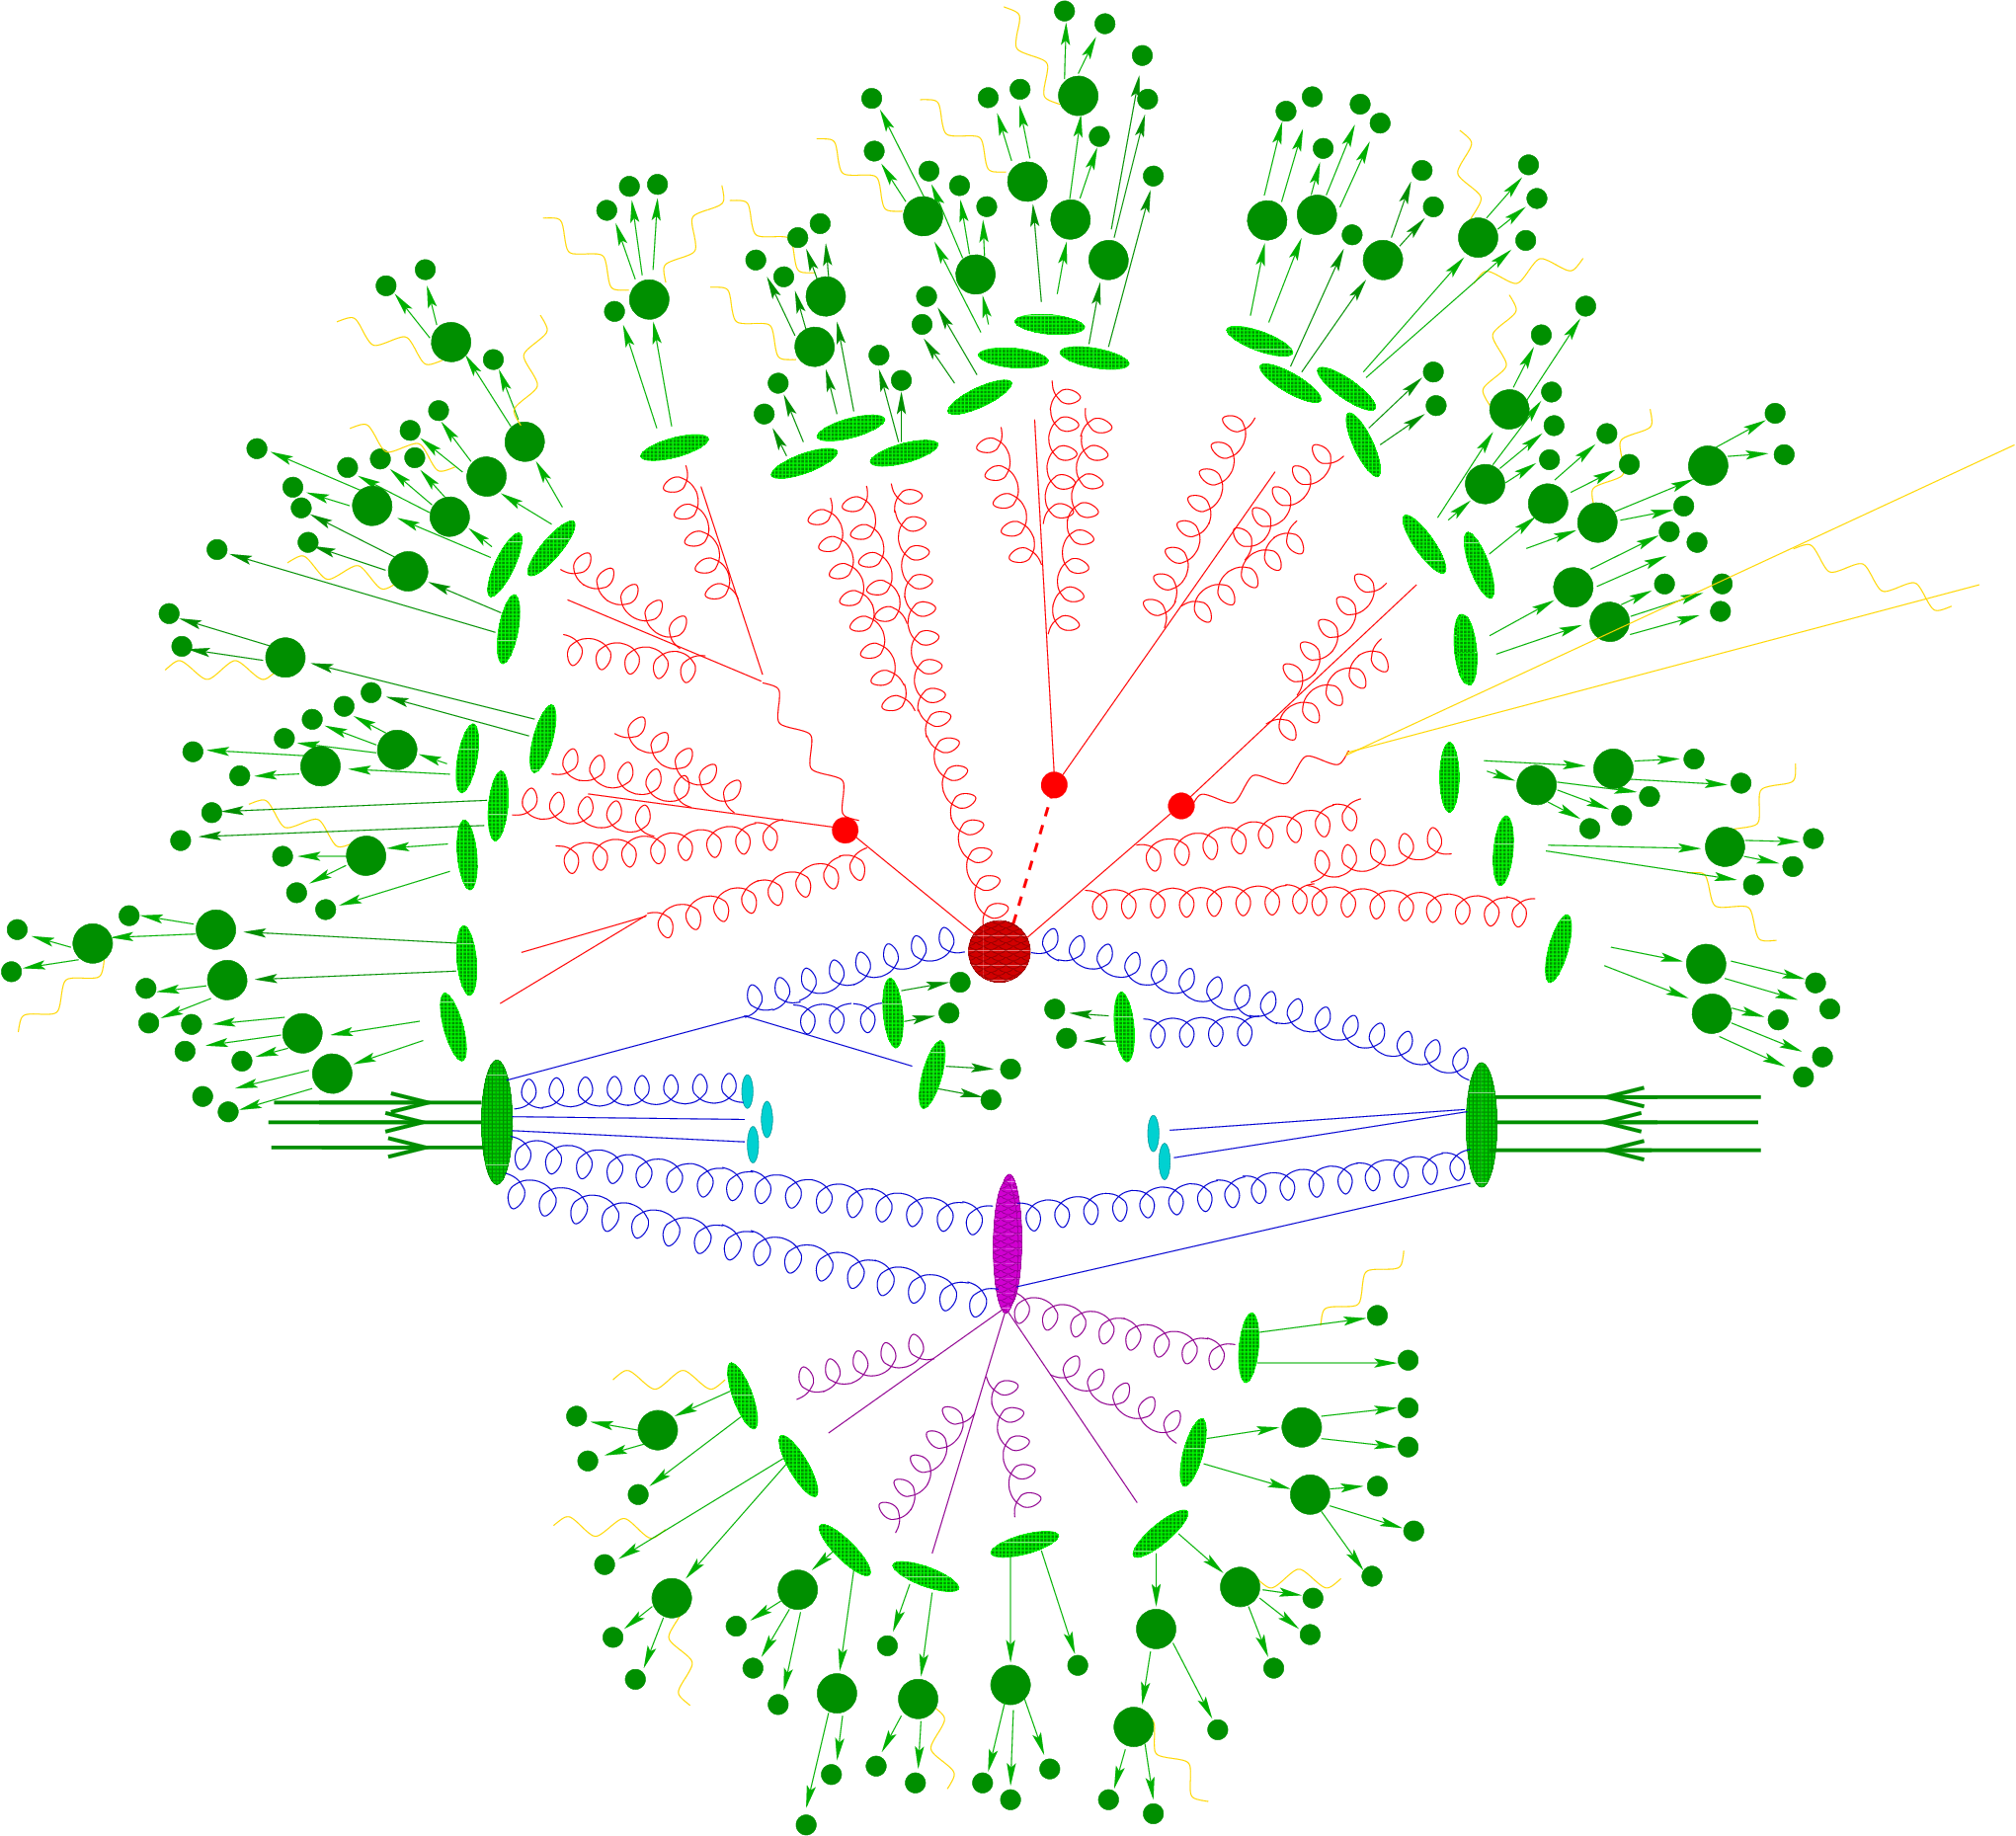
\includegraphics[width=0.6\textwidth]{sherpa_event}}
\end{figure}

\improvement{simulation tools allow to plugin any Lagrangian and get events at detector level}

The majority of $pp$ collisions are not interesting for particle physicists in the sense that they only involve soft hadrons travelling along the beam axis. Only a few events actually involve an \textit{hard-scattering} event with high-momentum transfer, rendering them interesting for particle physicists to study. Generating and understanding the final states of these $pp$ collision events is an enormously challenging problem as it typically involves hundreds of particles with energies spanning many orders of magnitude~\cite{Buckley:2011ms}. This makes the matrix elements connected to these processes too complicated to be computed beyond the first few orders of perturbation theory. The treatment of divergences and the integration over large phase-spaces further complicates the calculation of experimental observables.

It is not surprising that the simulation of the hard-scatter interaction is at the heart of any \gls{mc} event generator. Due to the high-momentum transfer scale, the cross section of this process can be calculated perturbatively using collinear factorisation~\cite{Buckley:2011ms},
\begin{equation}
	\sigma = \sum_{a,b}{\int_0^1{\diff x_a \diff x_b\int{\diff\Phi_n f_a^{h_1}(x_a,\mu_F) f_b^{h_2}(x_b,\mu_F)} \times \frac{1}{2 x_a x_b s}\vert \mathcal{M}_{ab\rightarrow n} \vert^2 (\Phi_n; \mu_F,\mu_R)}},
\end{equation}
with $x_a$ and $x_b$ the momentum fractions of the partons $a$ and $b$ with respect to their parent hadrons $h_1$ and $h_2$, $\mu_F$ and $\mu_R$ are the unphysical factorisation and the renormalisation scales, respectively and $\diff\Phi_n$ is the differential final state phase-space element. The phase space integration is typically done using \gls{mc} sampling methods. The choices for $\mu_R$ and $\mu_F$ are to some degree arbitrary, but are typically chosen to be in accordance with the logarithmic structure of \gls{qcd}, such that the matrix elements can be combined with the subsequent parton showers~\cite{Buckley:2011ms}. The \gls{me} $\vert\mathcal{M}_{ab\rightarrow n}\vert^2$ can be calculated using different methods~\cite{Buckley:2011ms}, with most \gls{mc} generators employing \gls{lo} computations. As \gls{lo} matrix elements are only reliable for the shapes of the distributions, an additional \textit{K-factor} correcting the normalisation of the cross section to \gls{nlo} is typically used. The probability of finding a parton with momentum fractions $x$ in a hadron $h$, is given by the \gls{PDF} $f_a^{h}(x,\mu_F)$ and depends on the probed factorisation scale $\mu_F$. The \glspl{PDF} depend on non-perturbative aspects of the proton wave function and can thus not be calculated from first principles. Instead, they are extracted from measurements in deep inelastic scattering experiments (see \eg~\cite{Gribov:1972ri, Blumlein:1996wj}). The variety of \glspl{PDF} provided by different groups, is accessible in a common format through a unified interface implemented by the LHAPDF library~\cite{Buckley:2014ana}. In \gls{mc} generators, the choice of \glspl{PDF} not only play a crucial role for the simulation of the hard process, but also in the subsequent parton showers and multiple parton interactions, thus influencing both cross sections and event shapes.

Fixed-order matrix elements work well for describing separated, hard partons but is not sufficient to describe soft and collinear partons. Higher order effects from gluon radiation can be simulated using a \gls{ps} algorithm. The emitted gluons will radiate additional gluons or split into quark--antiquark pairs which can in turn undergo gluon radiation. The \gls{ps}  thus describes an evolutionary process in momentum transfer scales from the scale of the hard scatter interaction down to the infrared scale $\mathcal{O}(\SI{1}{\GeV})$ where \gls{qcd} becomes non-perturbative and partons are confined into hadrons. Both \gls{isr} and \gls{fsr} are simulated through the \gls{ps} . As opposed to \gls{me} calculations, \glspl{ps}  offer poor modelling of few hard partons, but excel in the simulation of collinear and soft multi-parton states.

In order to avoid double counting, the hard partons described by the calculation of the \gls{me} and the soft collinear emissions of the \gls{ps} have to be connected to each other. This is done either through \textit{matching} or \textit{merging}. \gls{me} matching approaches~\cite{Bengtsson:1986hr} integrate higher-order corrections to an inclusive process with the \gls{ps}~\cite{Buckley:2011ms}. Merging techniques like the CKKW~\cite{Catani:2001cc} or CKKW-L~\cite{Lonnblad:2001iq} methods define an unphysical merging scale which can be understood as a jet resolution scale such that higher order \gls{me} corrections are only calculated for jets above that scale (while jets below that scale are modelled with the \gls{ps}).

Next, additional activity in the event not directly associated to the hard process is simulated. The underlying event is typically defined to be all additional activity after \gls{isr} and \gls{fsr} off the hard process has been taken into account~\cite{Buckley:2011ms}. Furthermore, \textit{multiple interactions} can occur in a single $pp$ collision. The modelling of multiple interactions involves multiple hard scatter processes per $pp$ collision as well as multiple soft interactions in addition to the hard scatter process.

Once the \gls{ps} reaches energies of $\mathcal{O}(\SI{1}{\GeV})$, entering the non-perturbative regime of \gls{qcd}, the coloured objects need to be transformed into colourless states. This so-called \textit{hadronisation} step cannot be calculated from first principles but has to be modelled, typically with either a \textit{string} or a \textit{cluster} model. The most advanced of the string models is the \textit{Lund} model~\cite{Andersson:1983ia,andersson_1998}. It starts from linear confinement and considers a linear potential between a $q\bar{q}$ pair, that can be thought of as a uniform colour flux tube stretching between the $q$ and $\bar{q}$, with a transverse dimension of the order of typical hadronic size (\ie around $\SI{1}{\femto\meter}$). As the $q\bar{q}$ pair moves apart, the flux tube stretches in length, leading to an increase in potential energy, finally breaking apart once enough energy is available to create a new $q'\bar{q}'$ pair, resulting in two colourless quark pairs $q\bar{q}'$ and $q'\bar{q}$. The new quark pairs can again move apart and break up further, leading to quark anti-quark pairs with low relative momentum, forming the final hadrons. The cluster model is based on the preconfinement property of \glspl{ps} ~\cite{Amati:1979fg}, stating that the colourless clusters of partons can be formed at any evolution scale $Q_0$ of the \gls{ps}, and result in universal invariant mass distributions that depend only on $Q_0$ and the \gls{qcd} scale $\Lambda$, but not on the energy scale $Q$ or nature of the hard process at the origin of the \gls{ps}~\cite{Buckley:2011ms}. The universal invariant mass distribution holds in the asymptotic limit where $Q_0 \ll Q$. If further $Q_0 \gg \Lambda$, then the mass, momentum and multiplicity distributions of the colourless clusters can even be calculated perturbatively~\cite{Buckley:2011ms}. Cluster models start with non-perturbative splitting of gluons and $q\bar{q}$ pairs, followed by the formation of clusters from colour-connected pairs. Clusters further split up until the $Q_0$ scale is reached, where they form the final mesons.

 As not all hadrons formed in the hadronisation process are stable, the affected hadrons need to be decayed until they form resonances stable enough to reach the detector material. In addition \gls{qed} radiation, that can happen at any time during the event, needs to be simulated. This is typically done with algorithms similar to the ones used for the \gls{ps}.
 
 The simulation steps that cannot be performed from first principles but rely on phenomenological models (underlying event, \gls{ps}, hadronisation) introduce free parameters that need to be derived or \textit{tuned} from parameter optimisations against experimental data. In ATLAS, the output of \gls{mc} event generators is stored in so-called EVNT data format containing HepMC~\cite{Dobbs:2001ck} event records. Although only the stable final-state particles are propagated to the detector simulation, the HepMC event record contains the entire connected tree as so-called \textit{Monte Carlo truth}.
		
\subsubsection{Detector simulation}\label{sec:detector_simulation}

Only the final-state particles generated by the \gls{mc} event generator are read into the detector simulation. In ATLAS, the full detector simulation is handled \textsc{Geant4}~\cite{geant:2002hh}, a toolkit providing detailed models for physics processes and an infrastructure for particle transportation through a geometry. \textsc{Geant4} has knowledge about the full detector geometry as well as the materials used in the subdetectors and is able to compute the energy deposits (so-called \textit{hits}) from single particles in the different sensitive portions of the detector components. The \textsc{Geant4} simulation adds information to the Monte Carlo truth content created during the event generation, including however only the most relevant tracks (mostly from the \gls{id}) due to size constraints~\cite{Aad:2010ah}.

The complicated detector geometry and the detailed description of physics processes requires large computing resources for the full detector simulation using \textsc{Geant4}, rendering it inaccessible for many physics studies requiring large statistics. Several varieties of fast simulations are available to this end. One of the most-used ones is \textsc{ATLFAST-II}~\cite{Aad:2010ah} , a fast simulation that uses the \textsc{Geant4} full simulation only for the \gls{id} and \gls{ms}. The slow simulation in the calorimeters---that takes about 80\% of the full simulation time---is replaced with \textsc{FastCaloSim}~\cite{ATL-SOFT-PUB-2018-002}, using parameterised electromagnetic and hadronic showers. Compared to the $\mathcal{O}(\SI{e3}{\second})$ simulation time per event in the full simulation, the \textsc{ATLFAST-II} detector simulation only takes $\mathcal{O}(\SI{e2}{\second})$~\cite{Aad:2010ah}. 

\subsubsection{Digitisation}

During the digitisation step, the hits from the detector simulation are converted into detector responses, so-called \textit{digits} that are typically produced when currents or voltages in the respective readout channels rise above a certain threshold in a given time window. The digitisation considers a modelling of the peculiarities of each detector component, including electronic noise and cross-talk~\cite{Aad:2010ah}. The effects from out-of-time and in-time pile-up are also considered by reading in multiple events and overlaying their hits. In order to match the true pile-up distribution in data, the number of events to overlay per bunch crossing can be set at run time. As described in~\cref{sec:pileup}, effects from cavern background, beam halo and beam gas can either be mitigated or removed at analysis level and are therefore typically not simulated.








































 